%\documentclass[review]{elsarticle}
%\documentclass[preprint]{elsarticle}
%\documentclass[1p]{elsarticle}
%\documentclass[3p]{elsarticle}
%\documentclass[5p]{elsarticle}
\documentclass[final,5p,times,twocolumn]{elsarticle}
%\documentclass[final,5p,twocolumn]{elsarticle}

\usepackage[utf8]{inputenc} % Включаем поддержку UTF8
\usepackage[T2A]{fontenc}
\usepackage[english,russian]{babel}   % убрать русский перед отправкой статьи
\usepackage{lineno}
\usepackage{graphicx}
\usepackage{xcolor}
\usepackage[pdftex, backref, colorlinks]{hyperref}
\usepackage{multirow}
\usepackage{enumitem}

\modulolinenumbers[5]
%\journal{Journal of \LaTeX\ Templates}
%\journal{Journal}
\journal{Astroparticle Physics}

%%%%%%%%%%%%%%%%%%%%%%%
%% Elsevier bibliography styles
%%
%% `Elsevier LaTeX' style
\bibliographystyle{elsarticle-num}
%%%%%%%%%%%%%%%%%%%%%%%
%\hyphenpenalty=10000

%\setlength{\marginparwidth}{2cm}
\usepackage{todonotes}

%http://ctan.math.washington.edu/tex-archive/macros/latex/contrib/easy-todo/easy-todo.pdf
%\usepackage[enable]{easy-todo}


\begin{document}
\newcommand{\todoi}[1]{\todo[inline]{\Russian #1}}

%\listoftodos[Notes]
\tableofcontents  % пусть пока побудет, стереть перед подачей
\listoftodos[Notes]
\linenumbers

\begin{frontmatter}
\title{SPHERE-2 balloon experiment results.\\ Part I: EAS observations conditions
\todoi{Уточнить название статьи}}
%\title{EAS observation from the air in the SPHERE-2 experiment. \\ Part 1. Atmosphere monitoring.

\author[address1]{E.A.~Bonvech\corref{correspondingauthor1}}
\cortext[correspondingauthor1]{Corresponding author}
\ead{bonvech@yandex.ru}
\author[address1]{D.V.~Chernov}
\author[address1]{T.A.~Dzhatdoev}
\author[address2,address3]{M.~Finger Jr.}
\author[address2,address3]{M.~Finger}
\author[address4]{V.I.~Galkin}
\author[address4,address1]{D.A.~Podgrudkov}
\author[address1]{T.M.~Roganova}
\author[address4,address1]{I.A.~Vaiman}
\address[address1]{M.V. Lomonosov Moscow State University, Skobeltsyn Institute of Nuclear Physics (SINP MSU), Moscow, Russia}
\address[address2]{Charles University, Faculty of Mathematics and Physics, Prague, Czech Republic}
\address[address3]{Joint Institute for Nuclear Research, Dubna, Russian Federation}
\address[address4]{M.V. Lomonosov Moscow State University, Department of Physics, Moscow, Russia}

\begin{abstract}
The SPHERE-2 detector designed for the extensive air showers detection was developed and performed measurements in 2011--2013. The data the detector collected is still under analysis but here we present the analysis of the telemetry data and of the detector operation conditions including background lighting, temperature conditions and its effects, atmosphere studies.\todoi{переписать под фактическое содержание статьи.}
\end{abstract}

\begin{keyword}
primary cosmic rays\sep extensive air showers\sep Vavilov--Cherenkov radiation\sep balloon
\MSC[2010] 00-01\sep  99-00
\end{keyword}
\end{frontmatter}


\section{Introduction}
\todoi{Сделать акцент на глобальной цели эксперимента - максимально надёжном и аккуратном измерении потока КЛ без цели тщательного прописывания деталей спектра. Упомянуть Антонова как автора первой успешной реализации метода.}
The SPHERE-2 detector was designed for the primary cosmic ray (PCR) studies in the 10--1000~PeV energy range. The PCR particles induce the secondary particle cascades (extensive air showers, EAS) and secondary radiations (such as Cherenkov light, fluorescent light, radio emission) in the atmosphere that are registered by different methods by the ground-based detectors. However the SPHERE-2 experiment is a first successful implementation of a new EAS detection method --- detection of the reflected Cherenkov light using an aerial-based detector. 

This method, first proposed by E.~Chudakov~\cite{chu74}, allows, on one hand, to register EAS on the relatively large area and later reconstruct the Cherenkov photons lateral distribution function, and on the other hand, to utilize a small size compact detector with all the advantages of such setup. The mentioned advantages include (but are not limited to) the opportunity to implement: a complex topological trigger conditions prior to writing data to storage thus increasing the maximum operational count rate; direct on-line calibration system; high mobility with lower operational costs etc.

Common EAS ground-based arrays such as the Telescope Array~\cite{abu12}, Yakutsk EAS array~\cite{Yakutsk19} or the TAIGA~\cite{TAIGA20} detector are the ground-based structures that are spread over up to hundreds~\cite{abu12} square kilometers. Significant effort is needed in order to install sensitive elements of such vast arrays and to keep them network connected, power-supplied and time-synchronized. More effort is needed for the regular calibration of detector stations and atmosphere parameter control over vast area. 

On the other hand conventional imaging air Cherenkov telescopes (IACT, like HESS~\cite{HESS03a, HESS03b} or MAGIC~\cite{MAGIC16-1, MAGIC16-2}
%\todoi{ Ссылка на MAGIC 10.1016/j.astropartphys.2015.04.004 10.1016/j.astropartphys.2015.02.005}) 
are relatively compact systems that have good calibration means, high integrity power supply, atmosphere transparency control and so on.

Since the Cherenkov light from EAS has a very sharp directional pattern it can not be observed by detectors more than about 0.5--1~km far from the shower axis. Therefore the IACTs have relatively low upper energy threshold.

The compact detector that observes large surface area, however, can combine some strong sides of an IACT with high upper energy threshold. 

The general overview of the SPHERE-2 experiment can be found in~\cite{Ant15a}, and the detailed description of the detector electronics is given in~\cite{Ant20}.


%% сделать табличку параметр, точность измерения, диапазон измерения, интервал измерения (Бонвеч, Чернов)
%%% === Telemetry table === %%%
\begin{table*}[bth]
\centering
\caption{Telemetry sensors parameters}
%\todo[inline]{Нужно уточнить точность GPS}
\label{tab:telemetry_sensors}
%\href{https://docs.google.com/spreadsheets/d/1MEnVT2ue2mNZBabXCuhiacFWPkZbzGb2yeg4IZIXusI/edit?usp=sharing}{Table with telemetry parameters online} \\

\vspace{1pc}
\begin{tabular}{|c|l|l|c|r@{\hspace{1mm}}c@{\hspace{1mm}}l|c|}
\hline
\multicolumn{1}{|c|}{interval} & \multicolumn{1}{c|}{parameter} & \multicolumn{1}{c|}{data}  & \multicolumn{1}{|c|}{accuracy} & \multicolumn{3}{c|}{range}  & \multicolumn{1}{c|}{units} \\
%\hline
\hline
\multirow{6}{*}{1 sec} & \multirow{3}{*}{Detector position} &GPS altitude & 2 (1)* &  -1500&--&18000  & m a.s.l.\\
                                                      \cline{3-8}
                         &                              & GPS coordinates & 4 (2)** & &---&& m\\
                                                      \cline{3-8}
                       &                              & GPS time (PPS)& 1 & &---&& $\mu$s \\
                       \cline{2-8}
                       & \multirow{2}{*}{Detector orientation} & inclination angles (resolution) X,Y& 0.3 (0.02)&$-$25&--&25&deg\\
                                                      \cline{3-8}
                       &                              & compass azimuth (resolution) Z &2.5 (0.5)&0&--&360&deg\\
                       \cline{2-8}
                       &Control block                 & inner temperature& 1.5 & $-40$&--&70 &deg,$^\circ$C\\
\hline
\multirow{7}{*}{1 min} & \multirow{2}{*}{PMT status} & anode current & 0.03 & 0&--&125 & $\mu$A\\
                                                      \cline{3-8}
                       &                              & mosaic temperature & 1.5 & $-40$&--&70 & deg,$^\circ$C\\
                       \cline{2-8}
                       & Power source                 & high voltage (HV1) & 0.1 & 0&--&250 & V\\
                       \cline{2-8}
                       & \multirow{2}{*}{Barometer}   & pressure & 5 & 750&--&1100 & hPa\\
                                                      \cline{3-8}
                       &                              & temperature& 2 & $-20$&--&60 &deg,$^\circ$C\\
                       \cline{2-8}
                       & Balloon barometer            & pressure   & 3 & 0&--&1000 & Pa\\
                       \cline{2-8}
                       & Battery (19V)                & voltage & 0.01 & 0&--&40 & V\\
                       \cline{2-8}
                       & Constant voltage (5V)        & voltage & 0.01 & 0&--&40 & V\\
\hline
\multirow{5}{*}{10 min} & \multirow{3}{*}{PMT status} & first dinode voltage & 0.06 & 0&--&250 & V\\
                                                      \cline{3-8}
                       &                              & PMT temperature & 0.1 & -30 &--&50 & deg,$^\circ$C\\
                                                      \cline{3-8}
                       &                              & supply voltage & 0.006 & 0&--&25 & V\\
                       \cline{2-8}
                       & Trigger                      & counting rate &1&0&--&4& Hz\\
                       \cline{2-8}
                       & FADC boards                  & voltage (1.2, 2.5, 2.8) & 0.001 & 0&--&4 & V\\
\hline
\end{tabular}

\vspace{1mm}

\footnotesize \raggedright 
\hspace{6.5 mm}* 2 m accuracy according to the manufacturer provided data, 1 m accuracy according to our own analysis (see. in section~\ref{sect:orientation} )

\hspace{5 mm}** 4 m accuracy according to the manufacturer provided data, 2 m accuracy according to our own analysis (see. in section~\ref{sect:orientation} )
\normalsize
\end{table*}


\section{The SPHERE-2 detector \label{sect:detector}}

The \mbox{SPHERE-2} detector is a compact optical device to measure the EAS Cherenkov light from the balloon elevated to altitudes up to 1~km above the Earth snow covered surface. Special tethered balloon BAPA developed and created by Russian Augur agency for this experiment was used.

The \mbox{SPHERE-2} detector optics comprised a 1.5~m diameter spherical mirror with a 109 photomultiplier tube (PMT) mosaic. 

The PMT mosaic is located near the mirror focal surface and records the Cherenkov light reflected from the snow surface below the detector. PMTs are arranged in the hexagonal structure on the spherical surface (see details in~\cite{Ant20}, or below on Fig.~\ref{fig:2012-3_shore_image}). The central PMT of the mosaic is the Hamamatsu-R3686 photomultiplier and the others are the FEU-84-3 PMTs. The fields of view of PMTs are fixed in angular terms. The exact shape of the area that a single PMT observes depends on the PMT's position in the mosaic and the detector orientation.


\subsection{Control block telemetry}
% кратко, что меряем служебного в блоке электроники: ЦАП и АЦП, какие токи, какие температуры, где температуры.
% кратко про мозаику

The control block of the SPHERE-2 detector contained along with the main registration electronics (and power system) a large array of different sensors. These sensors located both inside and outside of the control block were used to monitor detector state and performance, collect supplementary data for the EAS measurements. The list of the sensors used, their measuring range, precision and data collection frequency is given in table~\ref{tab:telemetry_sensors}. 

The sensors inside the control block measured:
\begin{itemize}[nosep]
\item the temperature of the FADC boards (two sensors per boadrd) for cooling system operation;
\item the voltage on the secondary power supply units for PMT mosaic power stabilization;
\item the voltage and current on the main power supply unit;
\item the overpressure and temperature inside the balloon.
\end{itemize}
The sensors outside the control block measured:
\begin{itemize}[nosep]
\item detector position (GPS-module);
\item local air pressure and temperature;
\item compass.
\end{itemize}
Additional sensors were installed on the PMTs in the mosaic and controlled
\begin{itemize}[nosep]
\item power supply voltage;
\item anode current;
\item temperature.
\end{itemize}

Some data provided by these sensors was used to monitor the flight conditions and detector status in real time. Also, all the data was stored and later was used in EAS parameters reconstruction and in detector performance evaluation.


\subsection{Orientation control system}
\label{sect:orientation}
% описание датчиков (Чернов)

The detector axis at the rest state is oriented vertically and detector observes the snow covered lake surface just under the detector. During the measurements, the detector hanging under the balloon, swung and rotated freely. The detector inclination is an important factor for the shower parameters reconstruction as it determined the overall geometry of the experiment. To control the position and rotation of the detector an inclinometer and a magnetometer compass are installed on the PMT mosaic control board. 

The magnetometer compass measures the angle of the detector's orientation relative to the Earth's magnetic field with 0.1~degree precision.

The inclinometer measures two angles between it's internal orthogonal axes and the plane orthogonal to the gravity vector. The orientation of inclinometer axes respectively to detector mosaic axes was determined in the laboratory. After careful preparations the mosaic was set horizontally with precision better than $0.1^\circ$ and the zero level of the inclinometer was measured. All detector inclination angles were calculated considering recovered zero level.

The type of inclinometer used allows fast angles measurements with low power consumption, but, contrary to the gyroscopic ones, it is affected by acceleration. As we will see in sec~\ref{sect:telemetrydata} during detector flights there were no recorded strong wind gusts and the balloon position was stable. So we assumed that  registered by inclinometer angles were unaffected by swinging.

The GPS sensor Garmin 16xHVS~\cite{GPS-module-specs}, located on the control unit was used to measure geographical coordinates and an elevation above sea level. 

The GPS manufacturer declared the absolute accuracy of determining the coordinates of 4~m, and the altitude of 2~m. Our observations show than an accuracy of position detection by the GPS sensor differs for moving and stationary objects. 

The accuracy position determination of the GPS sensor in rest state was calculated from GPS data at a time when the detector was stationary on the lake ice. Daily distributions of the detector coordinates and altitude were plotted for 20 days in 2012 and 2013. The average sigma (actually the median) of these distributions is taken as the accuracy of the GPS sensor's determination: 2~m for coordinates and 1~m for altitude.

The accuracy of altitude determination by moving GPS will be considered in Sec.~\ref{sect:gps_correction}.

%%%% Какая есть телеметрия %%%%%
\subsection{Telemetry monitoring\label{sect:telemetry}}

During every experimental flight a lot of information about the detector status and the environmental parameters is recorded. The different telemetry data is received and checked every second, every minute and every 10 minutes. 

Every second the detector position and orientation was recorded. The GPS data of altitude, latitude and longitude, universal global time UTC, the angles of detector inclination by the inclinometer sensor, magnetometer compass data and the control block inner temperature was monitored. The additional GPS and barometer were deployed on the Baikal Lake ice surface level.

Every minute the PMT and the power status was monitored. Anode currents of all PMTs, the PMT mosaic temperature and the temperature of the PMTs high voltage power source as well as the voltage of the batteries and of constant voltage sources were recorded. Barometer sensors were polled every minute also.

Every ten minutes the PMT supply voltage, voltage at the first and tenth dinodes, temperature were checked for each photomultiplier. The measuring channel counting rates and voltage on the FADC boards with the measuring channels were also recorded.

\todoi{Описать в два слова, зачем оно тут в таком количестве регистрировалось}

\Russian{Данные с источников питания ФЭУ необходимы для оценки стабильности характеристик оптических модулей. Частота срабатывания дискриминаторов каналов используется для установки порогов. Отклонения значений питающих напряжения FADC от стандартных позволяют оперативно выявить неисправность измерительной электроники. Данные с датчиков температуры позволяют не только стабилизировать температуру внутри бокса с электроникой при помощи вентиляторов охлаждения, но и выравнивать температуру при включении внутреннего вентилятора.}

\section{Experimental conditions}
%\section{Site and weather}
\label{sect:data}
 
The SPHERE experiment was carried out on the Baikal Lake, Russia during winters 2008--2013. The Baikal lake ice thickness reaches 40--60~cm in February. The balloon launch pad was deployed on the frozen Baikal lake ice surface 700~m far from the shore in the point with coordinates near 51$^\circ$\,47'\,48''~N, 104$^\circ$\,23'\,19''~E. 
%51.796923~N, 104.388663~E http://www.google.com/maps?q=51.796923,+104.388663
%The balloon attracted the attention of a large number of Baikal tourists. 


\begin{table}[b]
\centering
\caption{The annual statistics of the SPHERE experiment on Baikal Lake\todoi{Done. Исправить количество триггеров 2008-2009}}
\label{tab:statistics}
\vspace{1pc}
\begin{tabular}{|c||c|r|c|r|r|}
\hline
run  & flights & PMT    & time, & triggers \\ 
year &         & number & hours & detected \\ 
\hline \hline
\multicolumn{5}{|c|}{test runs} \\
\hline
2008 & 1 &  20 &  1 &  6180 \\ 
2009 & 3 &  64 & 13 & 10312 \\ 
2010 & 6 &  96 & 30 &  1343 \\
\hline
\multicolumn{5}{|c|}{experiment runs} \\
\hline
2011 & 4 &  96 & 30 & 20571 \\
2012 & 5 & 109 & 31 &  7716 \\
2013 & 5 & 109 & 33 &  3813 \\
\hline
\end{tabular}
\end{table}


The \mbox{SPHERE-2} detector was lifted by the tethered balloon BAPA to altitudes up to 900~m above snow surface. The annual statistics of the experiment is given by the Table~\ref{tab:statistics}. The first two years were test ones. The detector configuration was improved from year to year. Thus the number of PMTs was increased from 96 to 109, the signal time sampling was changed in 2012 from~25 ns to 12.5~ns.

Unless otherwise specified, all illustrations in the paper are given for the \mbox{SPHERE-2} data of the winter 2013 run. All plots were made with Python Matplotlib plotting library.

%% Baikal snow photo %% fig:baikal_snow
\begin{figure}[tb]
    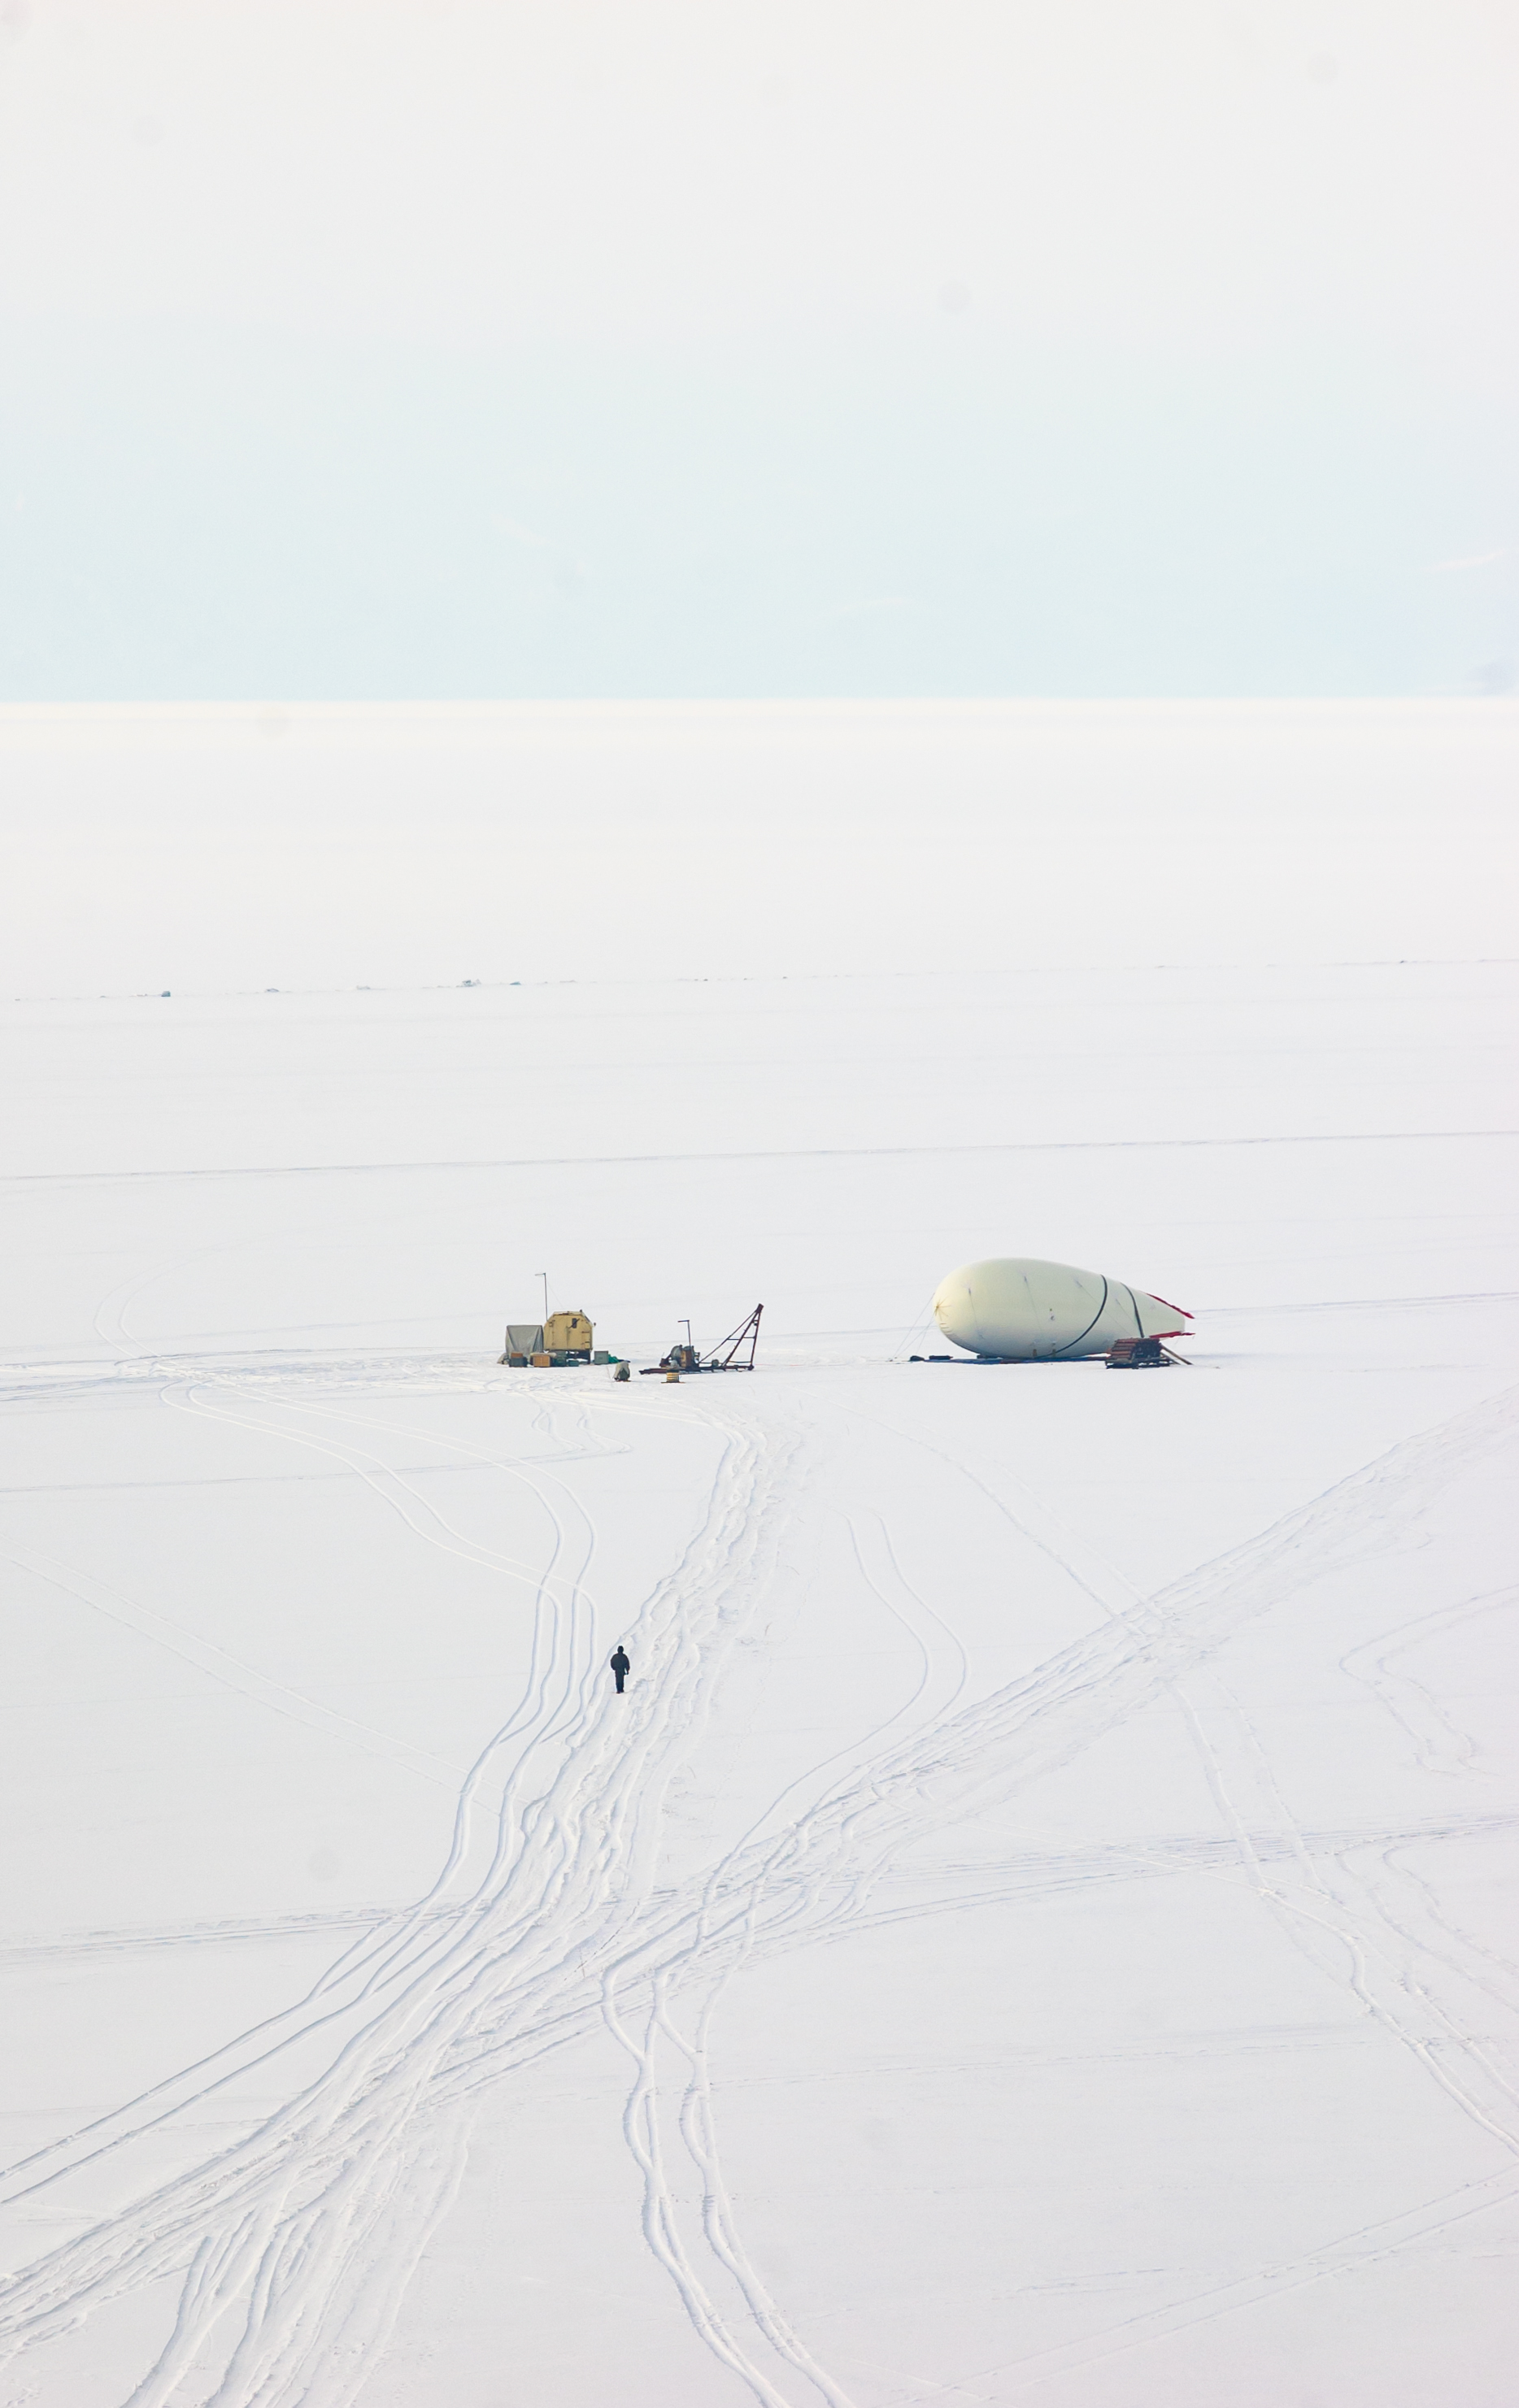
\includegraphics[width=0.45\textwidth]{figs/DSC_4049.jpg}\hspace{2pc}%
    \caption{Baikal snow around the SPHERE start point.}
\label{fig:baikal_snow}
\end{figure}

\subsection{Weather and snow}
% внести результаты собственного измерения условий на снегу

Measurements were carried out during clear moonless cloudless nights with low wind. The measurements were started 1.5 hour after sunset or immediately after moonset and were finished before moonrise or 1.5 hour before sunrise. If the wind condition had become unsuitable for the flight the balloon with detector was landed at once as it was in the third flight in 2013. The typical night air temperature on the lake surface was near $-15^\circ$C. According to~\href{https://rp5.ru/}{'Raspisaniye Pogodi'} data archive of the nearest weather stations with numbers 30818 and 30710 the horizontal visibility was at least 10 km, and the altitude of the base of the lowest clouds was 2500~m and more or no clouds were present. The Milky Way was clearly visible all the nights.

Our experiment was carried out when the Baikal surface was covered with freshly fallen snow. All the lake ice was covered by snow as seen in the Fig.~\ref{fig:baikal_snow}.  The snow reflection properties were controlled by using a luxmeter -- device sensitive to light intensity in the optical band. The influence of the snow state on its reflecting properties has been discussed in detail in our article on the simulation of the SPHERE-2 detector~\cite{Ant19}. 

\todoi{Наприсать про изменение погоды в/после 2013-5 со ссылкой на график плотности атмосферы.}

\subsection{Detector orientation and telemetry data\label{sect:telemetrydata}}

The \mbox{SPHERE-2} detector position and wind conditions near the detector are clear from the Fig.~\ref{fig:gps_compass} and Fig.~\ref{fig:inclination}. The Fig.~\ref{fig:gps_compass} demonstrates every minute \mbox{SPHERE-2} detector coordinates according to GPS sensor during flights of 2013 winter run. The start point is located at zero coordinates. The detector orientation measured by magnetometer is indicated by arrows. Figure~\ref{fig:gps_compass} demonstrates that wind was quite constant and the balloon position was rather stable. The balloon position was affected by the wind. But the detector orientation was stable in the wind flow and it rotated around its axis slowly during all the experiment.  

%% detector drift figure %% fig:gps-compass
\begin{figure}[tb]
    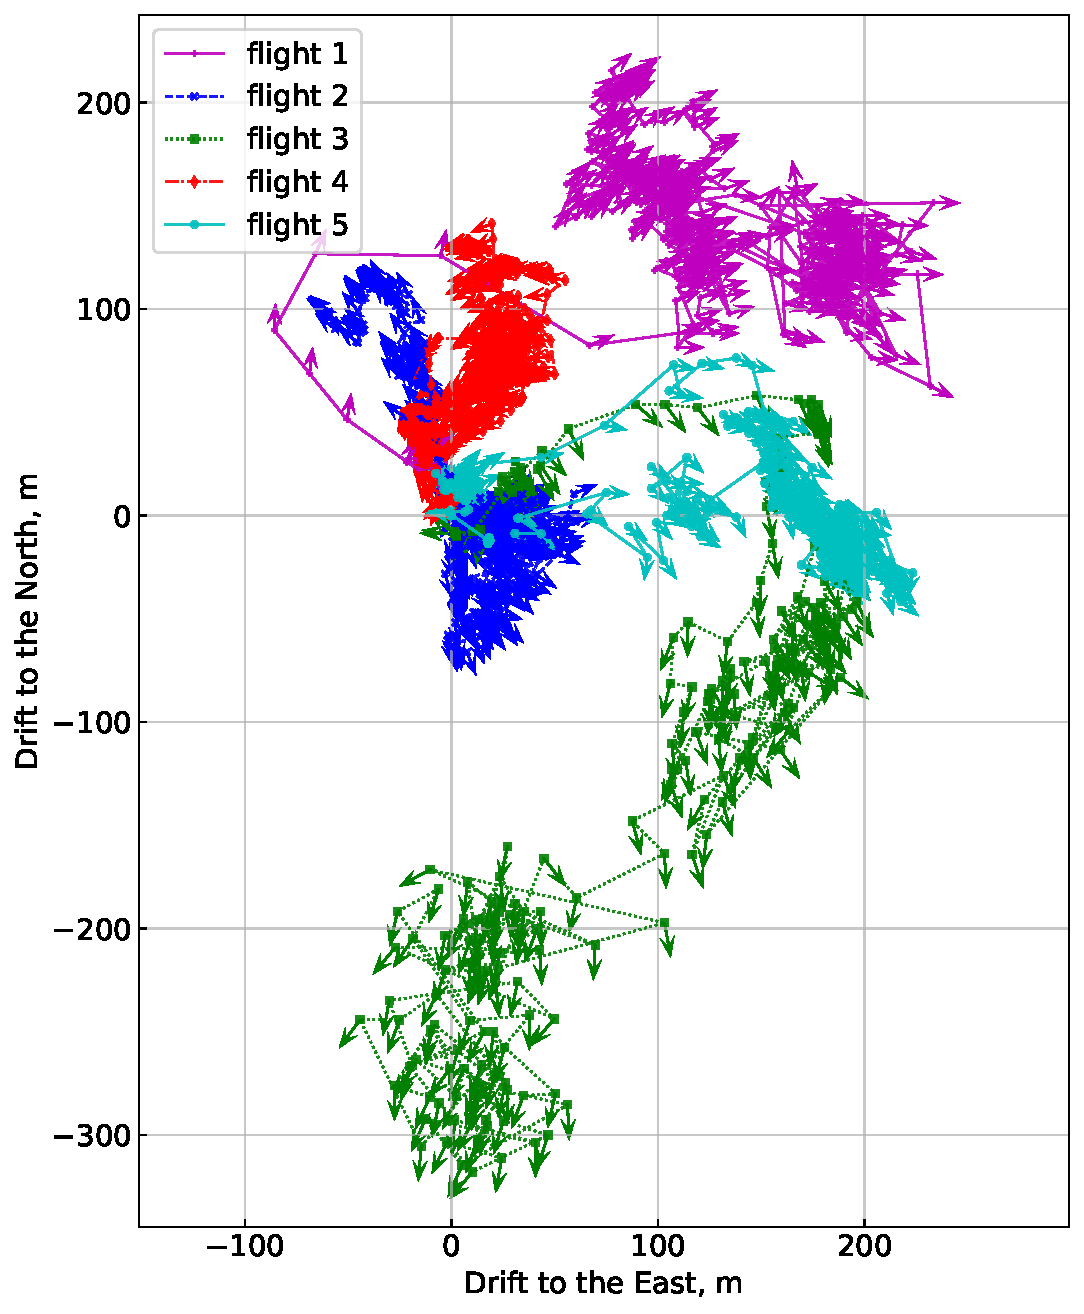
\includegraphics[width=0.45\textwidth]{figs/GPS+quiver.pdf}\hspace{2pc}%
    \caption{The SPHERE-2 detector drift in 2013. The arrows indicate the detector magnetometer orientation. The start point is located at zero coordinates.}
\label{fig:gps_compass}
\end{figure}

Under the influence of wind the SPHERE-2 detector was deflected by a small angle from the vertical axis. For example, as one can see on the Fig.~\ref{fig:inclination} in 2013 run during second and fourth flights the~\mbox{SPHERE-2} detector was suspended almost vertically, while in the others it was tilted by the wind but this declination was steady and varied slowly over time. The maximum inclination angle of the detector was about twenty degrees from vertical axis. The inclination effect was taken into account at the stage of EAS parameters reconstruction.

Fig.~\ref{fig:height} shows the detector altitude above lake ice surface according to the GPS module data. The surrounding air temperature and pressure are presented on the Fig.~\ref{fig:temperature} and Fig.~\ref{fig:pressure} respectively according to the data of the onboard pressure sensor.

%%  4 telemetry  pictures %%%
\begin{figure*}[tb]
    \begin{minipage}[t]{0.48\textwidth}
    \centering
    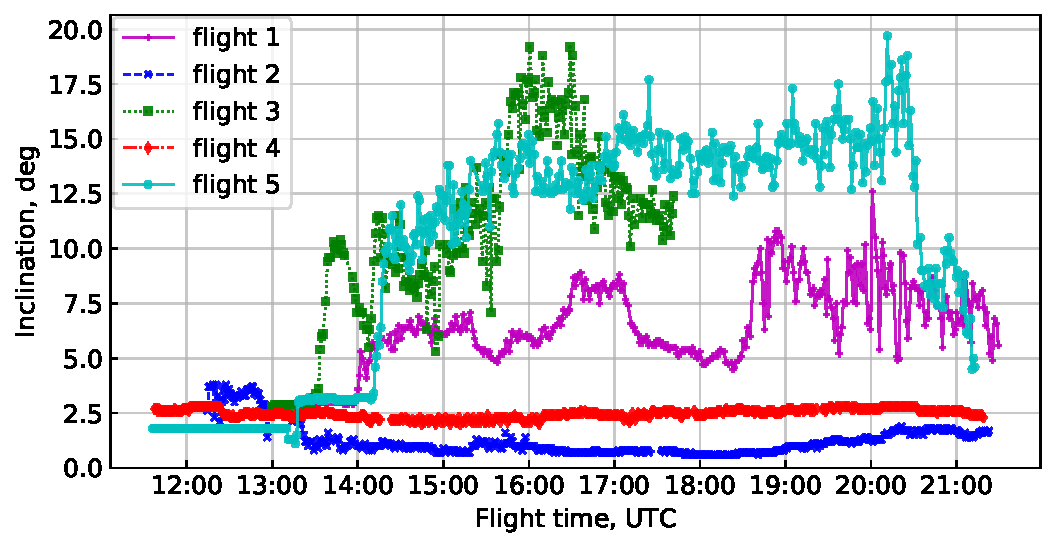
\includegraphics[width=\textwidth]{figs/ClinTh.pdf}
    \caption{The detector inclination during 2013 experiment run according to the inclinometer data.}
    \label{fig:inclination} 
    \end{minipage}
    \hfill
    \begin{minipage}[t]{0.48\textwidth}
    \centering
    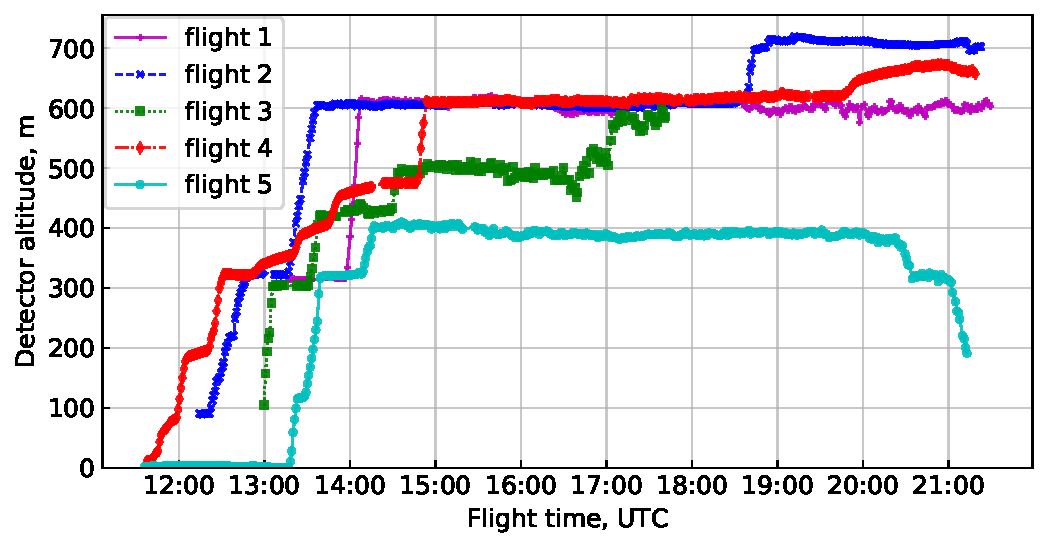
\includegraphics[width=\textwidth]{figs/height.pdf}
    \caption{The altitude of the SPHERE-2 detector carried by the BAPA tethered balloon during 2013 experiment run according to the GPS module data.}
    \label{fig:height}
    \end{minipage}
    
    \vspace{\baselineskip}
    
    \begin{minipage}[t]{0.48\textwidth}
    \centering
    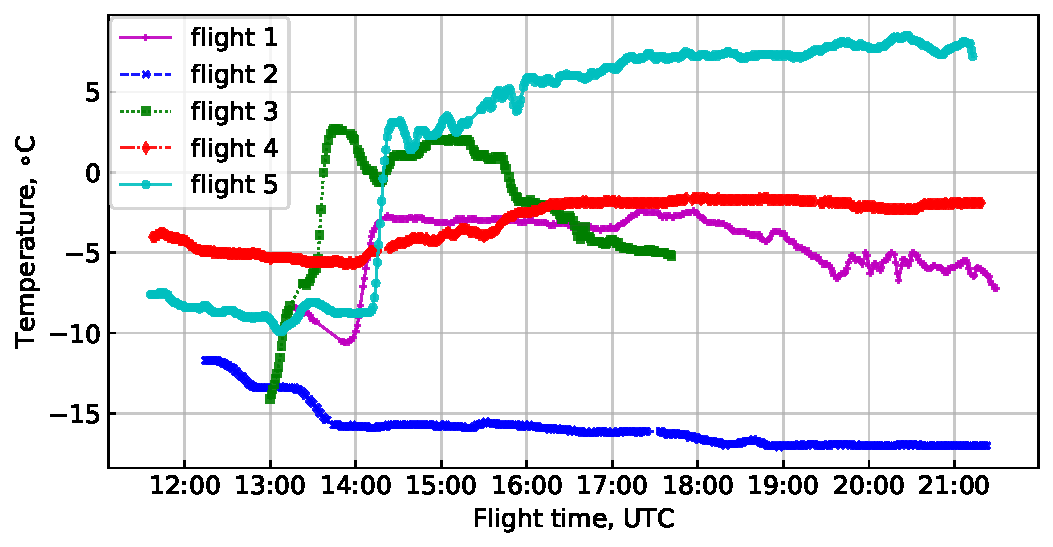
\includegraphics[width=\textwidth]{figs/T1.pdf}
    \caption{The air temperature during 2013 run according to the barometer sensor data.}
    \label{fig:temperature}
    \end{minipage}
    \hfill
    \begin{minipage}[t]{0.48\textwidth}
    \centering
    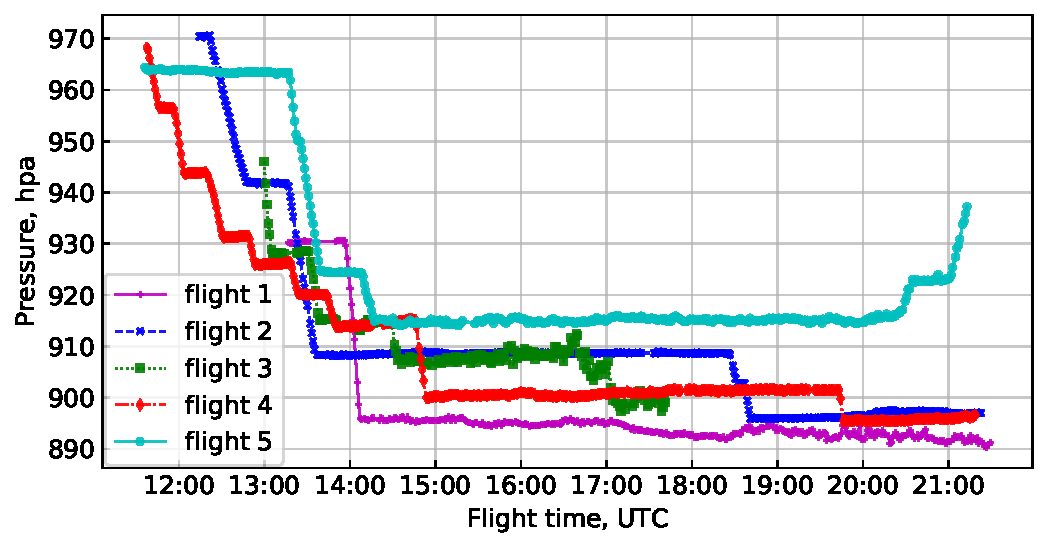
\includegraphics[width=\textwidth]{figs/P_hpa0.pdf}
    \caption{The air pressure during 2013 flights according to the barometer sensor data.}
    \label{fig:pressure}
    \end{minipage}
\end{figure*}
%%%%%%%%%%%%%%


%% radius-inclination
\begin{figure}[tb]
    %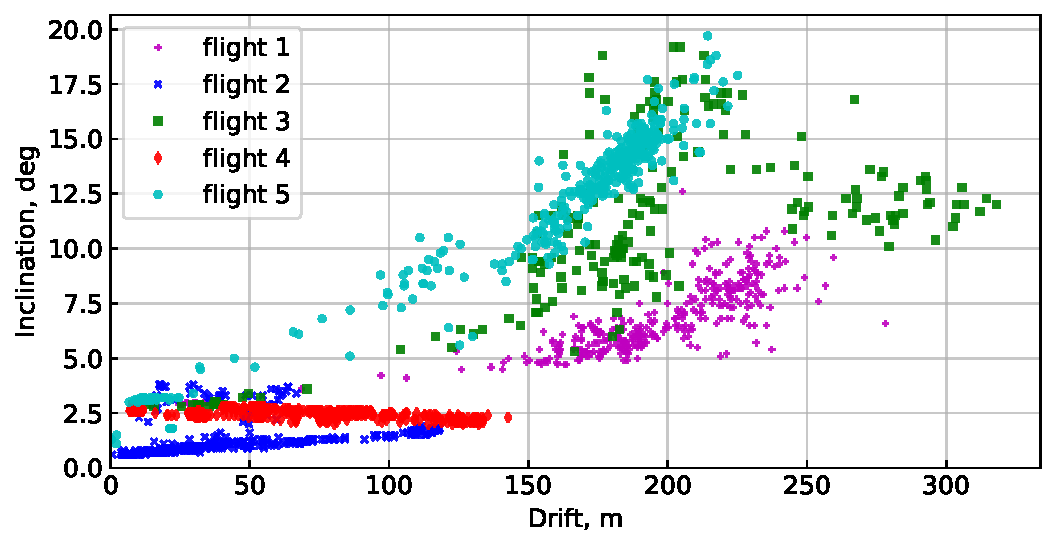
\includegraphics[width=0.48\textwidth]{figs/radius-inclination.pdf}
    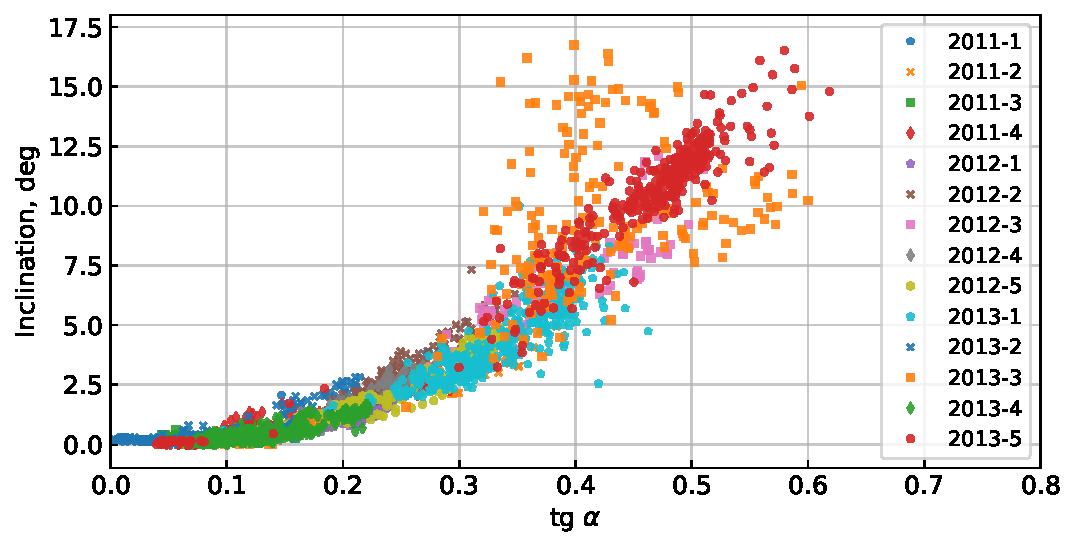
\includegraphics[width=0.48\textwidth]{figs/tg-inclination.pdf}
    \caption{Detector inclination vs the detector drift from the start point to the detector altitude ratio which roughly translates into the tether inclination angle.}
\label{fig:drift-inclination}
\end{figure}


\subsection{PMT currents and background light}

%% The central PMT current
\begin{figure}[tb]
    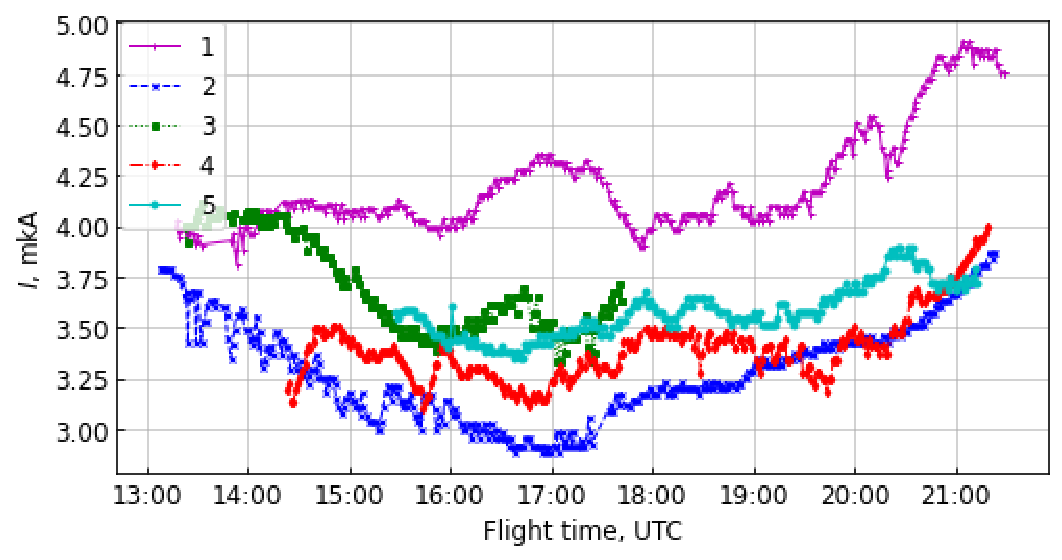
\includegraphics[width=0.48\textwidth]{figs/cur2013_PMT1.pdf}
    \caption{The central PMT currents in flights of 2013.}
\label{fig:current}
\end{figure}

The PMT currents (the average anode current) were monitored constantly during flights as a part of detector state control. Since some of the PMTs used in the detector exhibited strong gain dependence on background illumination (up to a factor of 2) during initial selection and testing prior to the detector assembly the in-flight currents were expected to vary with time.

In principle, the PMT anode current contain the current from photoelectrons and from thermoelectrons. However, in total dark conditions (in the laboratory during testing and at a launch site in the light protected storage container) the registered currents were small, below currents measurement precision. Therefore in-flight currents were considered as being caused only by photoelectrons from snow background illumination.\todoi{Прописать подробнее про токи в ящике и в лаборатории.}

The background light flux was calculated as the sum of the few time-dependent fluxes from different sources, each with its own time dependence. Moreover each source of background light has its own spectrum that in theory can change over time due to atmosphere absorption.

The main contributors to the total flux in 180--1000~nm wavelength range are:
\begin{enumerate}
    \item airglow --- the emission of light by variety of recombination and photochemical processes in the upper layers of atmosphere caused by its partial ionisation by Sun ultraviolet light and CR;
    \item zodiacal light --- the Sun light back-scattered by the interplanetary dust cloud originating (mostly) from the Jupiter-family comets~\cite{Nesvorn__2010};
    \item planets --- being the brightest sky objects during the 2011--2013 seasons the give noticeable addition the the total light flux;
    \item stars and deep sky objects --- the fluxes from these two contributors cannot be easily separated since the limited resolution of the telescopes and optical overlapping of the relatively nearby dust and gas clouds and unresolved faint stars.
    \item light pollution --- the combined scattered light from artificial sources;
\end{enumerate}

The airglow has a complex spatial wave structure due to its mechanism of origin. But on average the sky has an almost constant airglow brightness of 21.9$^m$ per square second of arc in V band (see, for example,~\cite{BENN1998503}). For these calculations the airglow spectrum was taken as a set of [OI] and [NaI] lines (558, 589, 630 and 636~nm) that lay within the SPHERE PMTs sensitivity region~\cite{Ant16}. The [O2] presudo-continuum was not included into calculations since it has a very low total flux even near the maximum of PMTs sensitivity. The relative brightness of each line was taken from~\cite{KRASSOVSKY1962883}. The average airglow brightness variation dependence on the solar activity was taken from~\cite{BENN1998503}. The solar 10.7-cm radio flux was taken from National Research Council Canada archive of daily observations. The dimming of certain lines at the end of astronomical twilight was not simulated since all the measurements with the SPHERE detector were performed well after the end of the astronomical twilight. For the whole night the brightness of the airglow was considered to be constant.

The zodiacal light brightness model was taken from~\cite{BUFFINGTON201688}. The model was somewhat simplified: non-analytical residuals (parts $E$ and $F$) were not included in the calculations due to them being unavailable. Plus, we had to change the equation for $h$ to simple $(180-\gamma')$ to get correctly looking results (e.g. same distribution as in Fig.~C1 of the original publication). Was that due to the misprint in the original publication or our own deep code error was never found. The zodiacal light being a scattered light has a Sun spectrum and was approximated by a black body spectrum with 6000~K temperature. The general night variation of the total zodiacal light flux was estimated relative to the UTC time. The calculations were performed in the ecliptic coordinates  to simplify calculations by skipping the coordinates transformation since the trajectory of the zenith point in these coordinates is easy to find for any given date relative to that years equinox. 

The planets are among the brightest objects on the night sky, therefore they should be included in calculations. For calculations only Venus, Mars, Jupiter and Saturn

The light pollution from all sorts of artificial sources was estimated using data from ``The new world atlas of artificial night sky brightness''~\cite{Falchie1600377} as being around 10~\% of the natural background. The spectrum of artificial sources in the area was of the two major types: incandescent light sources (households illumination) and high pressure sodium-vapor lamps (city street lights). However, in the area of the Baikal lake the first type does give a negligible flux compared to the second type. The second source type has a set of bright wide lines. For these calculations we took high pressure sodium-vapor lamps emission spectrum from~\cite{Elvige2010}. The spectrum of the back-scattered and partially absorbed light that actually lit the snow surface far from the areas of its origin was modified proportionally to the Rayleigh scattering cross section and absorption by 3 full atmospheres (since the launch site was located about 30--55~km away for relatively large urban areas of Irkutsk, Baikalsk and Slyudyanka).

Current of the central PMT is shown on the Fig.~\ref{fig:current}. 



\todoi{Дописать!}
%%%%%%%%%%%%%%%%%%%%%


\subsection{PMT currents variations}

%% 2012-3 currents
\begin{figure}[t]
    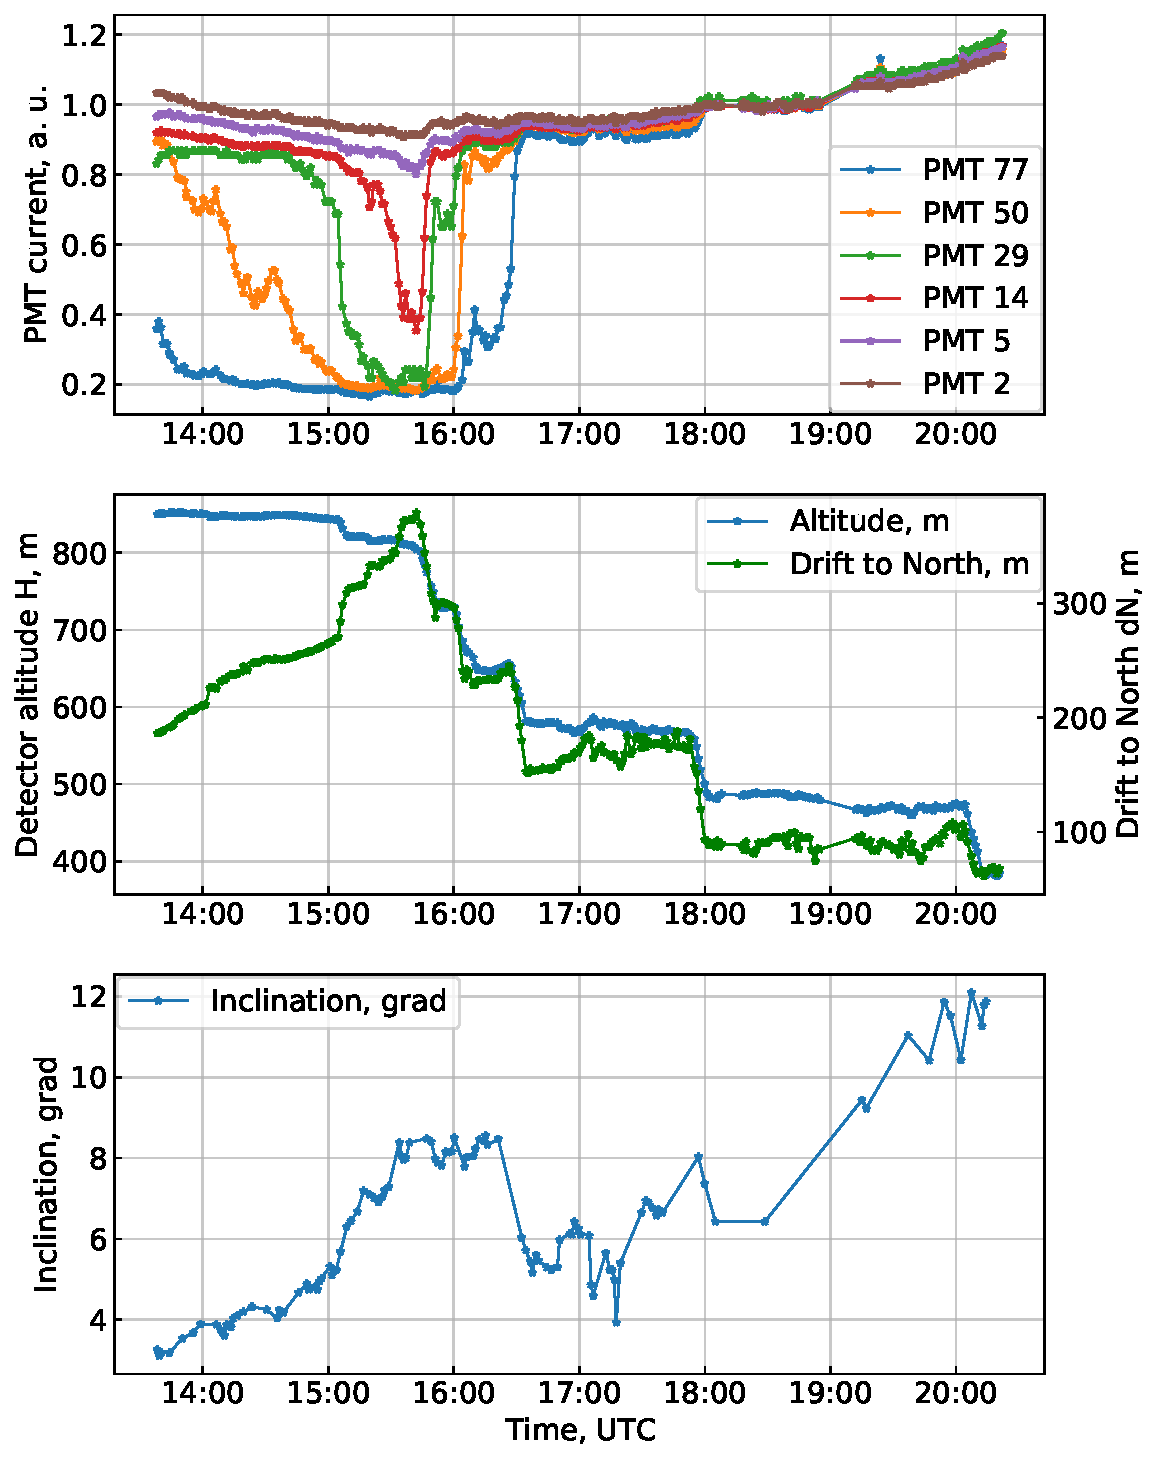
\includegraphics[width=0.48\textwidth]{figs/2012-3_currents_H_dN.pdf}
    \caption{PMT currents, detector drift to the North, altitude and  inclination during flight 2012-3.}
    \label{fig:2012-3_currents}
\end{figure}

\begin{figure}[tb]
    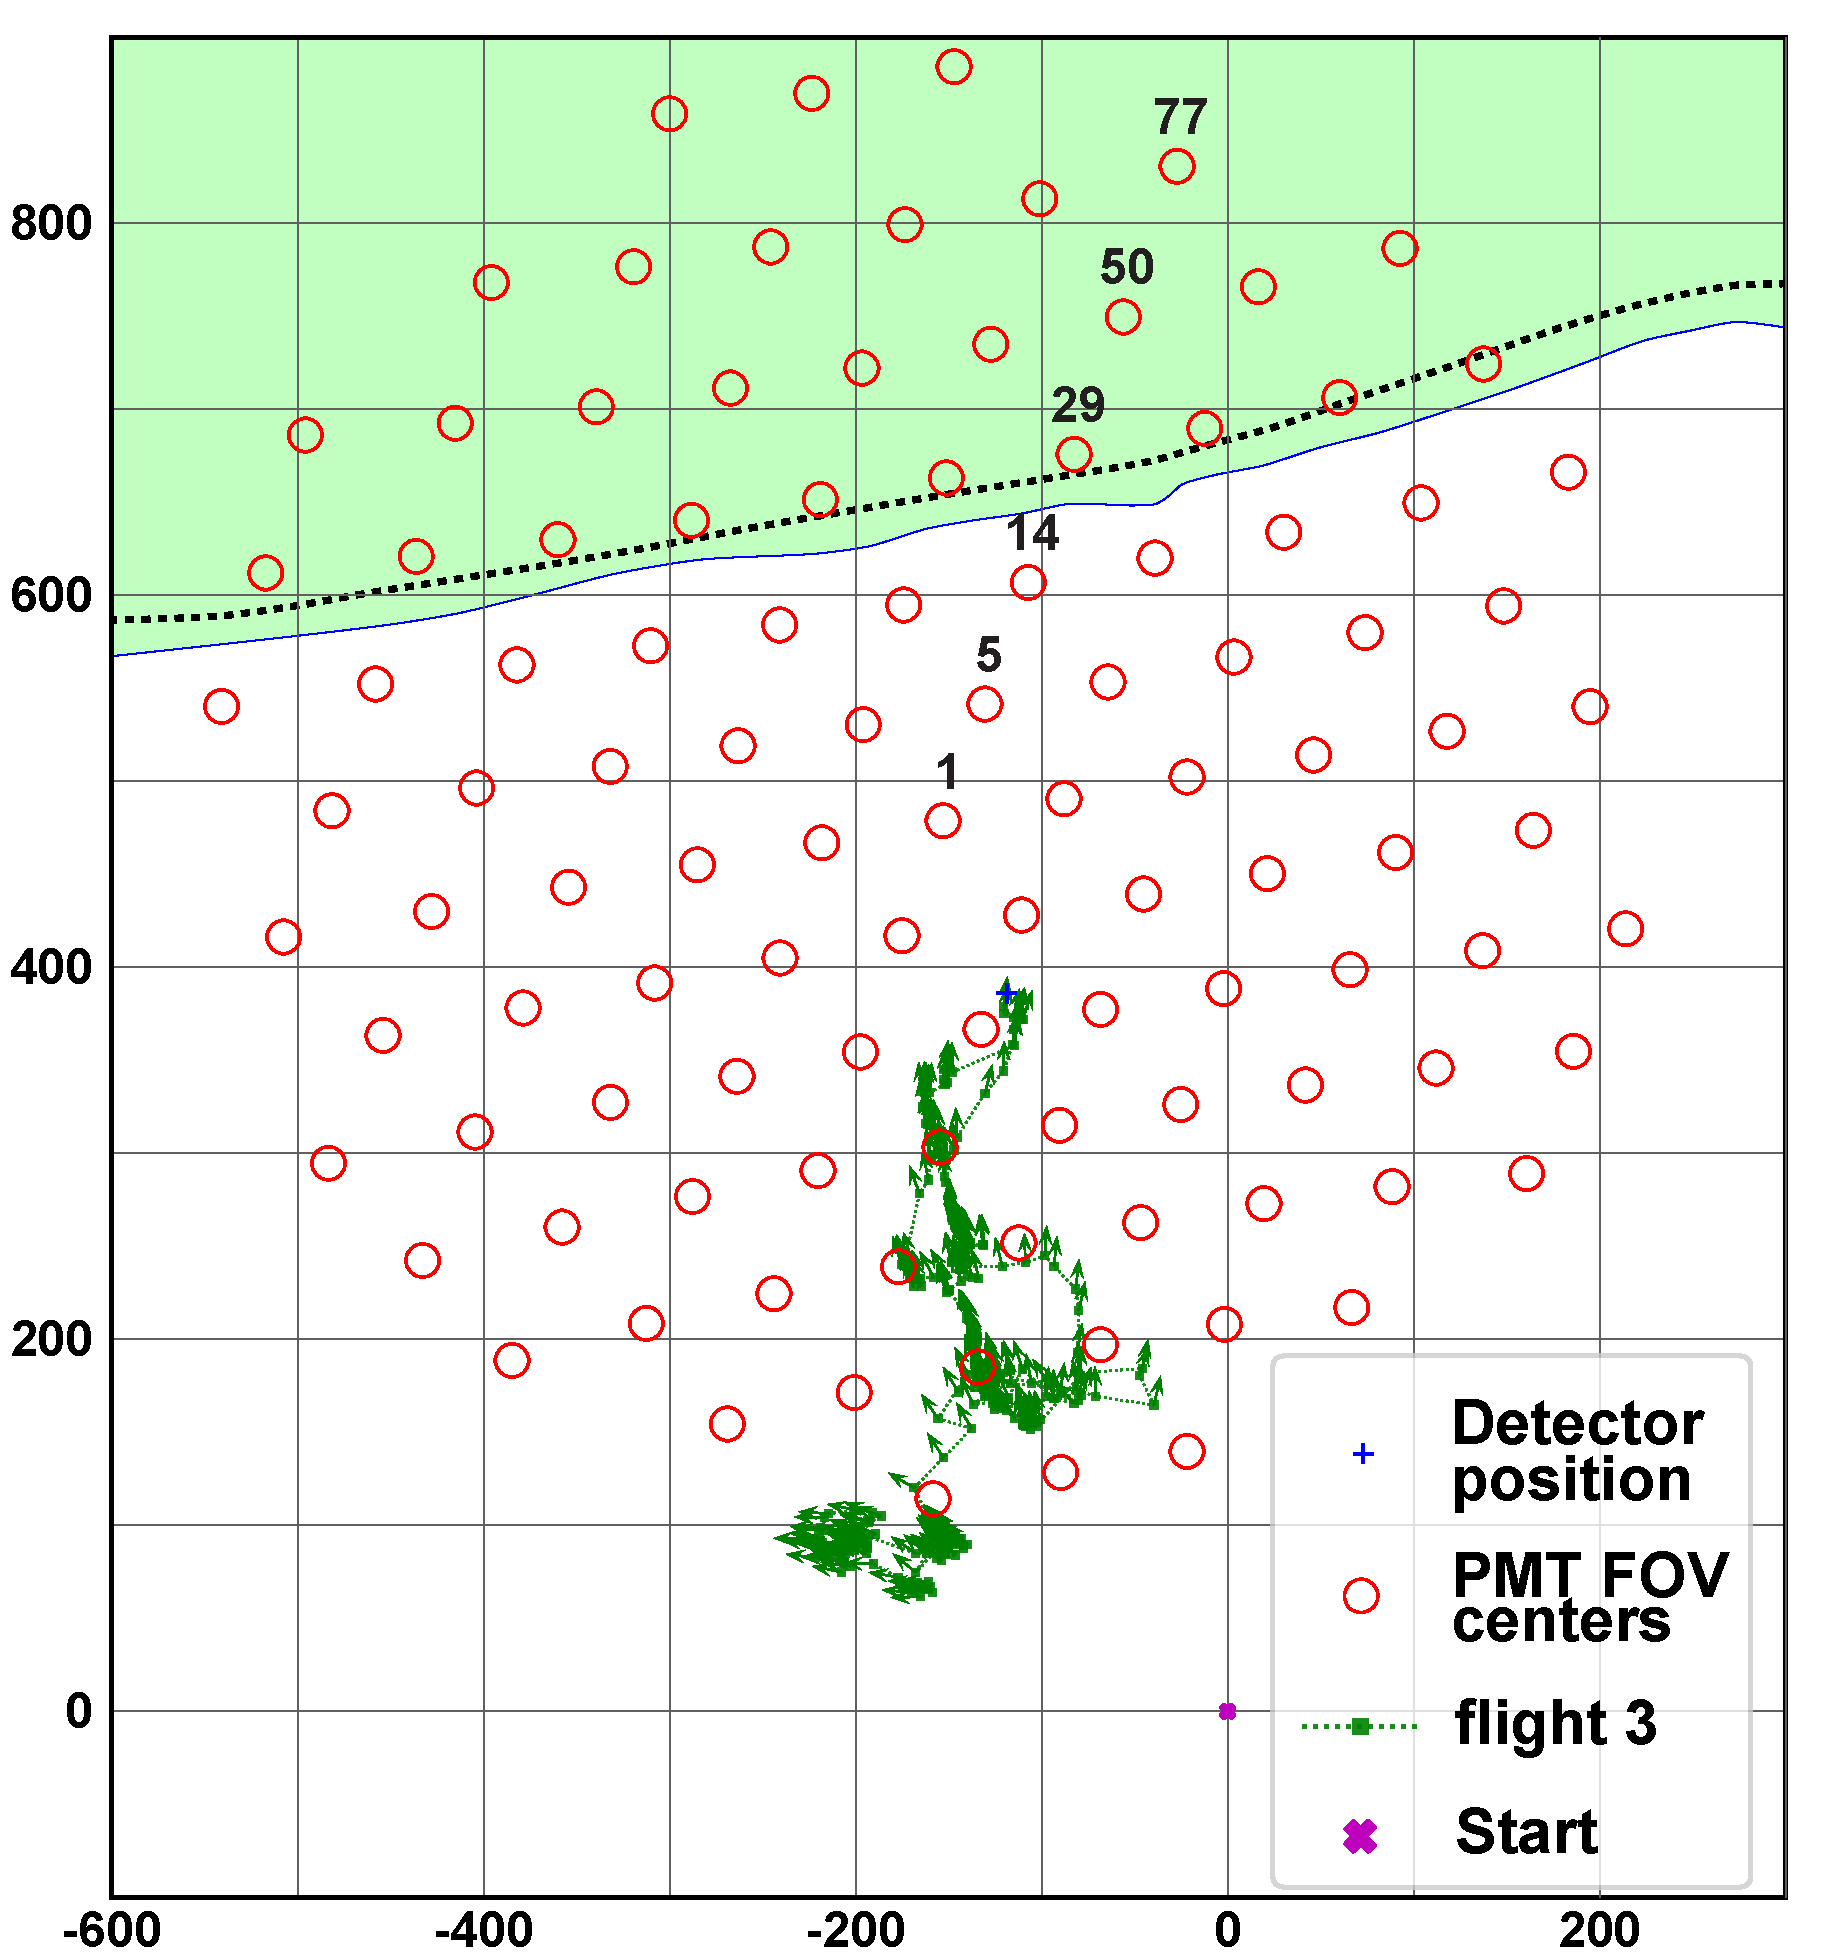
\includegraphics[width=0.48\textwidth]{figs/2012_drift-mod.pdf}
    \caption{The SPHERE-2 detector drift in 2012-3 flight. Retina projection to the show surface is given for the time 15:47 UTC. Detector GPS position at that moment is indicated by the cross.}
    \label{fig:2012-drift}
\end{figure}


The PMTs currents variations during the observations generally followed the variation of the background illumination of the snow. However, in third flight of the 2012 season in part of the PMTs the abnormal drop of currents was observed (see Fig.~\ref{fig:2012-3_currents}).

\begin{figure}[tb]
\centering
    %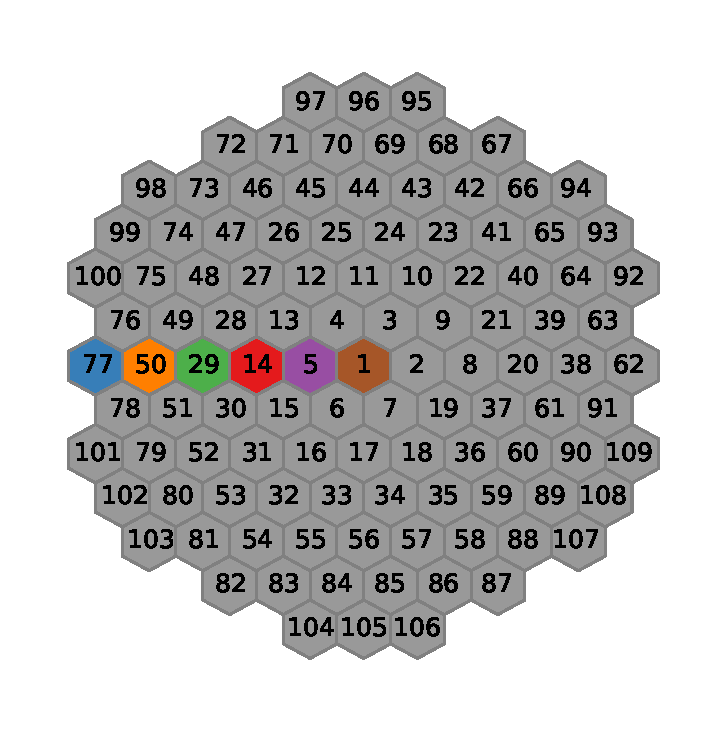
\includegraphics[width=0.2\textwidth]{figs/2012-3_retina.pdf}
    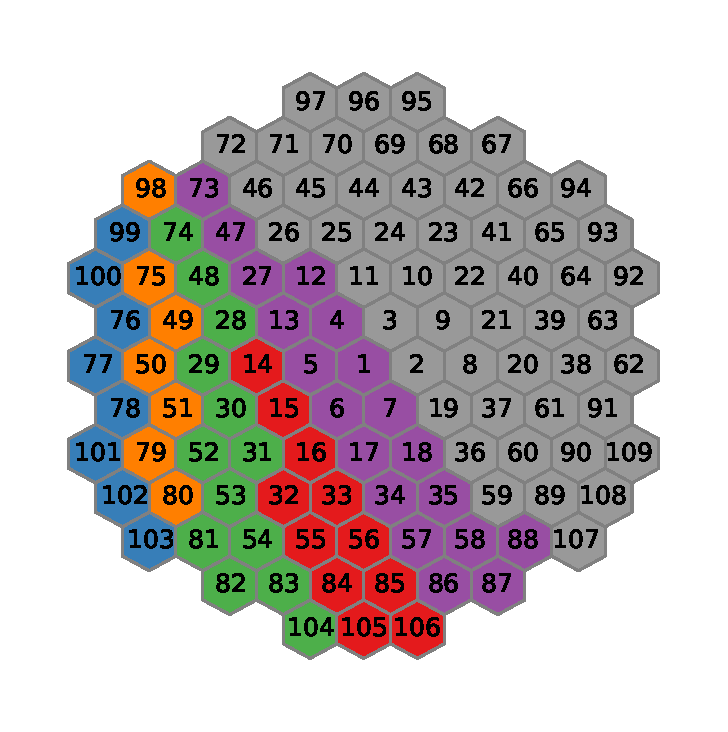
\includegraphics[width=0.35\textwidth]{figs/2012-3_retina_all.pdf}
    \caption{The SPHERE-2 PMT mosaic scheme. PMT numbers are indicated. PMTs are colored according to it current curve type in 2012-3 flight with colors as in Fig.~\ref{fig:2012-3_currents}.}
    %\todoi{Выберите одну из двух.}
    \label{fig:2012-3_shore_image}
\end{figure}

The registered currents in some PMTs (numbers 5, 14, 29, 50 and 77) are shown in Fig.~\ref{fig:2012-3_currents}~(top panel). These PMTs form a straight line on the PMT mosaic and the currents dropped and restored in them in the same order they are positioned in the mosaic. There were more PMTs with current drop occurring at the same time. In Fig.~\ref{fig:2012-3_shore_image} the PMTs are colored according to similar current drop and restore times.

This anomaly was observed in the the first half of the flight during the observations at 850~m altitude. At that time according to GPS the balloon was drifting north from starting point. Detector altitude and drift see in Fig.~\ref{fig:2012-3_currents}~(central panel). Due to the wind becoming stronger on that altitude the balloon was subsequently lowered to 480 altitude and the currents had returned to their normal behaviour. 

the analysis of the position and tilt of the detector showed that 
\todoi{Не закончено.}
%В первой половине третьего полета в 2012 наблюдалось необычное снижение токов в некоторых измерительных каналах. Оно наблюдается при высоте аэростата свыше 700 м над озером и сносе аэростата до 400~м на север. На рис~\ref{fig:2012-3_currents} в одних временных координатах представлены: токи, снос на север и высота детектора над поверхностью озера, надо еще добавить угол наклона установки. На верхнем рисунке~\ref{fig:2012-3_currents} приведены токи для фотоумножителей из центрального ряда мозаики ФЭУ: с 77 по 2 согласно нумерации фотоумножителей на рис.~\ref{fig:mosaic}. Согласно данным компаса мозаика была ориентирована таким образом, что ФЭУ 77 осматривало наиболее северную часть поверхности поля зрения всей установки. ФЭУ в легенде на рис.~\ref{fig:2012-3_currents} перечислены в порядке расположения полей зрения с севера на юг. Чем более южную часть обозревает ФЭУ, тем эффект ослабления тока меньше как по длительности, так и по абсолютной величине. Изменение тока ФЭУ коррелирует по времени с изменением сноса на север. 

%Зная очертания береговой линии озера Байкал и исходя из данных телеметрии, мы делаем вывод, что такое уменьшение токов обусловлено тем, что под действием ветра на высоте более 700~м аэростат с детектором сносился к северу рис.~\ref{fig:2012-drift}, детектор наклонялся в сторону севера, в поле зрения ФЭУ попали участки суши, покрытые темными деревьями. Установка частично смотрит на тёмный берег, а не на снег озера, поэтому токи уменьшились. Чем дальше на север сдвигалась установка, тем более дальний от края ФЭУ видел уменьшение тока.  

%Потом аэростат спустили пониже, снос стал меньше и в поле зрения всех ФЭУ остался только снег. 

%При этом есть ФЭУ, например, PMT2 на рис.~\ref{fig:2012-3_currents}, которые все время смотрят только на снег и видят отраженный от него звездный свет. Временной ход тока в таких ФЭУ можно объяснить общим изменением засветки атмосферы, ну или еще чем-нибудь и Дима это обязательно сделает. 

%}



\section{Telemetry analysis}
%%% Переименовать и пересортировать

The position and inclination of the SPHERE-2 detector are the important values to correct calculations of detected EAS Cherenkov light characteristics. In contrast to ground-based Cherenkov light installations, the detector SPHERE-2 has a variable recording area depending on both the altitude and the inclination angle of the detector.

%%%%%%%%%%%%%%%%%%%%%%%%%%%%%%%%%%%%%%%%%%%%%%%%%%%
\subsection{GPS altitude correction with barometer data}
\label{sect:gps_correction}

Thorough telemetry data analysis reveals that at some periods of time recorded GPS data for altitude is inadequate. Namely, after sudden changes in altitude due to balloon ascent or descent, GPS height lags behind corresponding pressure change and varies in a smoothed fashion. The example of such behavior is shown in Fig.~\ref{fig:h_corr}, top panel. We were unable to find out the exact source of this distortion, but our best guess is that it's a result of GPS module's internal error correction algorithm. Module's primary application is naval navigation~\cite{GPS-module-specs} and it may interpret sudden change in altitude as an error.

\begin{figure}[tb]
    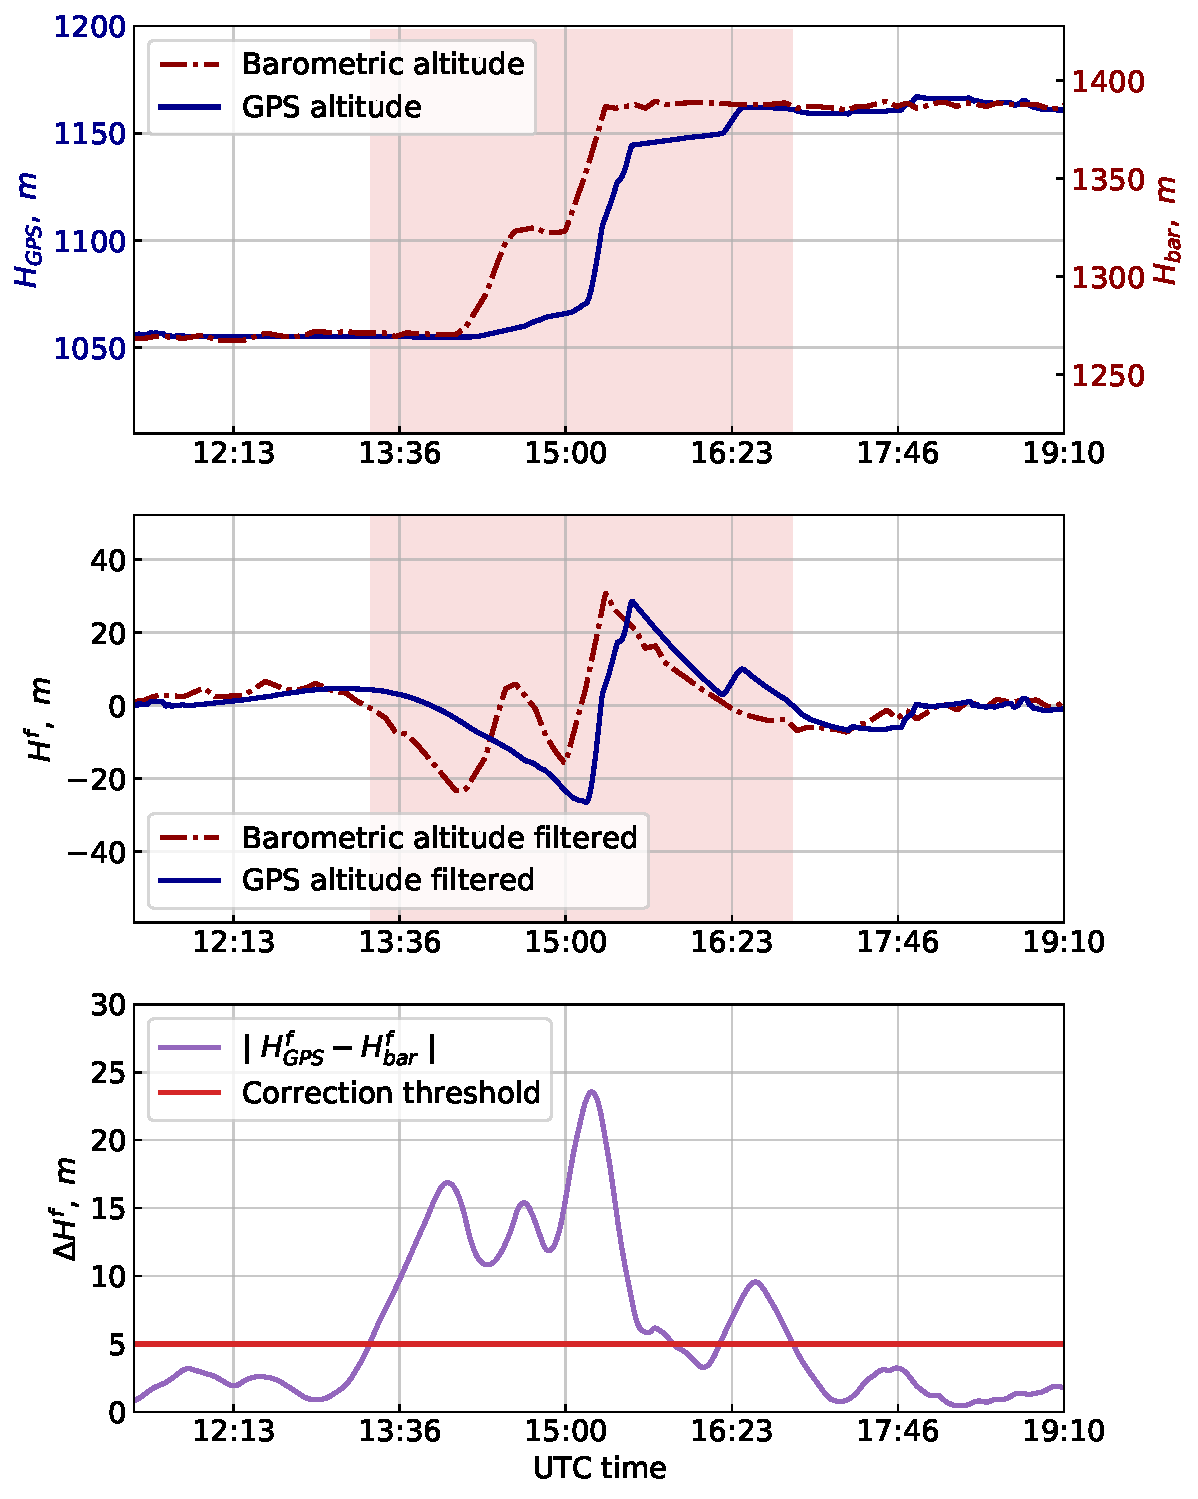
\includegraphics[width=0.48\textwidth]{figs/height_correction.pdf} 
    \caption{Example of anomalous GPS altitude behavior, compared with `barometric' altitude (top panel). Same data with high-pass digital Butterworth filter applied (middle panel). Smoothed absolute delta of high-passed altitudes from middle panel, used as gate with threshold set at red line; intervals above this line correspond to red bands on other panels, which are the intervals subjected to GPS data correction.}
\label{fig:h_corr}
\end{figure}


\begin{figure}[t]
    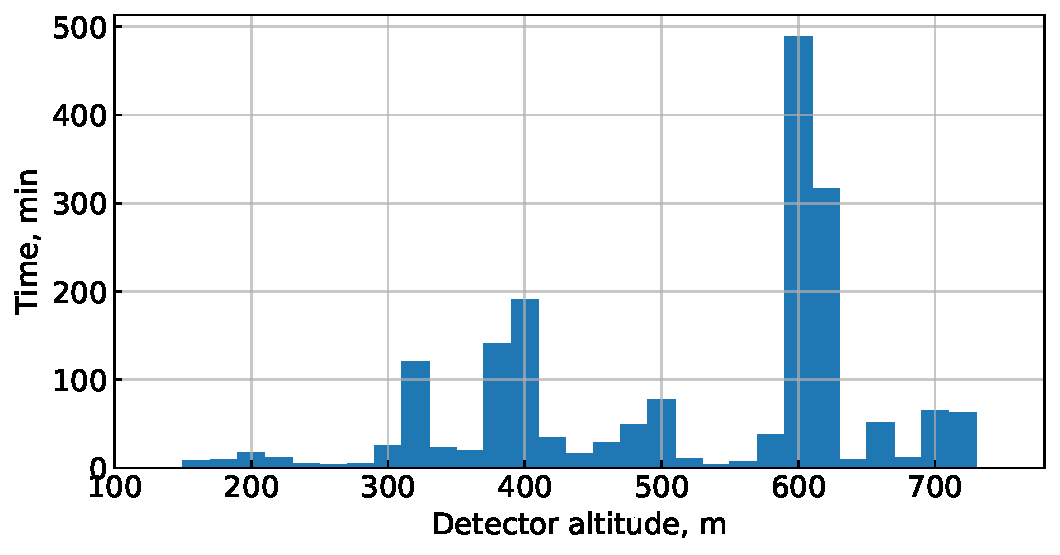
\includegraphics[width=19pc]{figs/time_on_altitude.pdf}%
    \caption{The altitude distribution of experiment time.}
    \label{fig:time_on_altitude}
    \todoi{Описать картинку в тексте. Обновить картинку по исправленным высотам.}
\end{figure}

Affected time intervals are relatively short for most flights, but during them some (сколько?) events were recorded. In order to correctly estimate detector altitude for those events, and to maintain overall data consistency we attempted to correct these smoothed GPS altitude measurements using pressure data from barometer, which has strong and well-understood dependence on altitude.

First of all, to identify affected time intervals we calculated approximate <<barometric height>> from pressure data using inverted barometric formula $H_{bar} = H_0 - a \log \frac{P}{P_0}$ with parameters $H_0 = 456~\textrm{м}$ (Baikal surface level), $P_0 = 1000~\textrm{hPa}$ (close to average March pressure on the Baikal surface) and $a = \frac{RT}{Mg} \approx 8400~\textrm{m}$ (standard value for barometric formula). Next, we have applied a high-pass digital Butterworth filter to both GPS and barometric altitude data to compare only fast variations of both values. Cutoff frequency for filter was set to $0.416~\textrm{mHz}$ ($T=40$ min with telemetry data being recorded each $10~\textrm{sec}$) and slope was set to around $12~\textrm{db per octave}$. Resulting high frequency components are shown on Fig. \ref{fig:h_corr}, middle panel.

It is clear that for stable altitude and valid GPS measurements GPS and barometric height are subjected to fast, somewhat correlated fluctuations (they are not completely correlated probably due to GPS error of the order of several meters). In contrast, intervals of smoothed GPS data show divergence of these two values. We calculate delta between filtered GPS and barometric altitudes and apply moving average with $6~\textrm{min}$ window. We then define intervals subject to correction as those that feature the smoothed delta above a threshold of $5~\textrm{m}$ in absolute value. The threshold is chosen so that in regular conditions the smoothed delta is doesn't exceed it, as it has normal-like distribution with standard deviation of around $3~\textrm{m}$. Smoothed delta with the threshold are shown in Fig \ref{fig:h_corr}, bottom panel; correction interval is shown on top panel with red band.



After intervals are picked, for each of them we find two adjacent intervals $2~\textrm{min}$ each with correct GPS data and once again use barometric formula to estimate actual altitude inside the interval. In this case it is used to describe local behavior of $H(P)$. We fit $(P, H)$ data points from adjacent regions with the same barometric function and replace smoothed GPS data with the new <<local barometric height>>.

After the corrections to GPS altitude data had been made we estimated the atmosphere density profile.

%%% Atmosphere profiles figures %%%%
\begin{figure}[bt]
\centering
\begin{minipage}[t]{0.48\textwidth}
    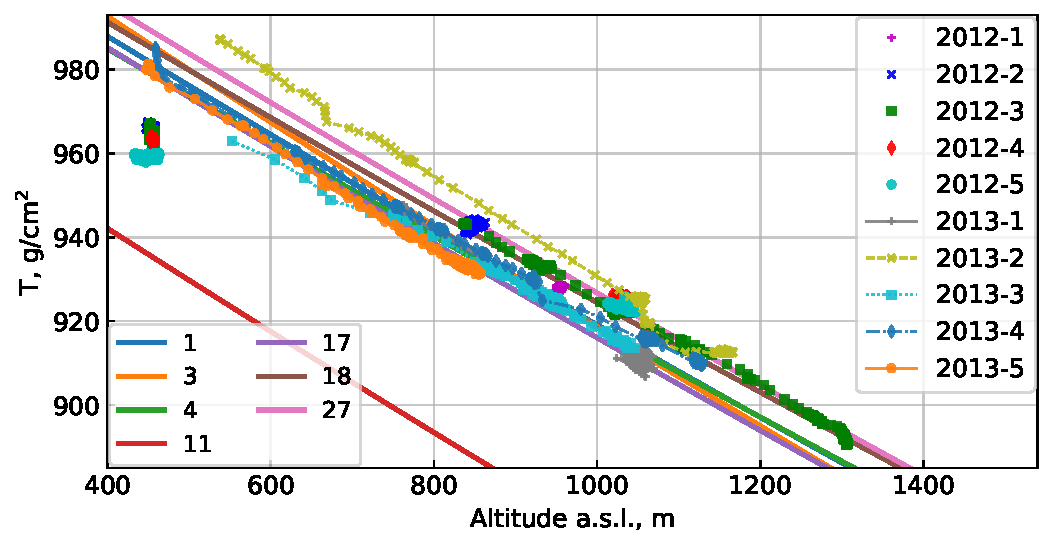
\includegraphics[width=\textwidth]{figs/atmosphere_T.pdf}
    \vspace{-1.0pc}
    \caption{Mass overburden versus altitude points in each flight and CORSIKA profiles. Solid black line represents profile adopted in the preliminary modelling}
\label{fig:massoverburden}
\end{minipage}
\vfill
\vspace{1pc}
\begin{minipage}[t]{0.48\textwidth}
    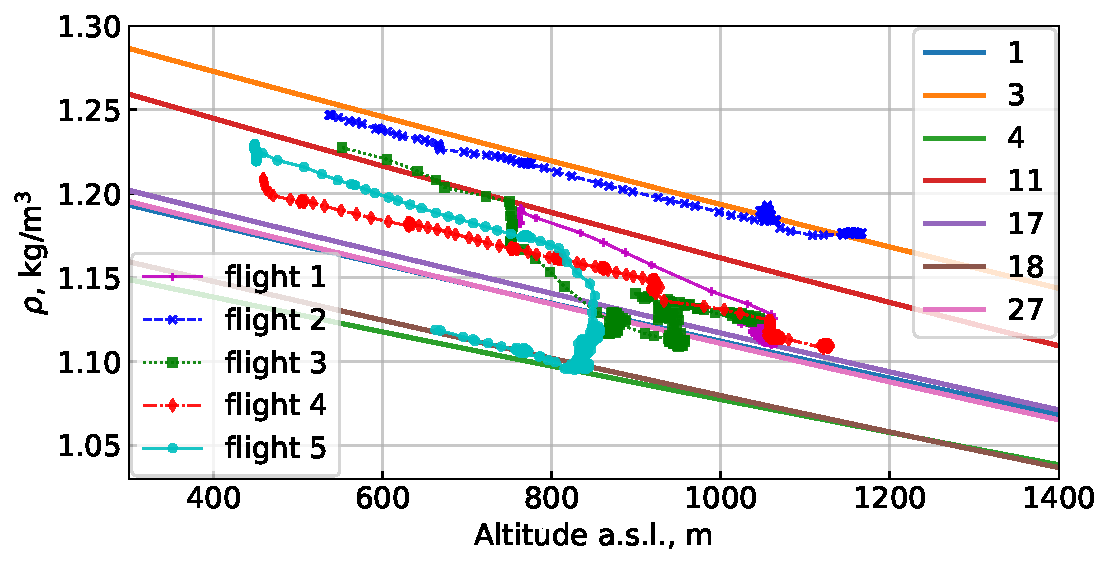
\includegraphics[width=\textwidth]{figs/atmosphere_rho.pdf}
    \vspace{-1.0pc}
    \caption{Density versus altitude points in each flight and CORSIKA density profiles (negative derivatives of the curves in Fig. \ref{fig:massoverburden}). Solid black line represents profile adopted in the preliminary modelling}
    \todoi{Добавить данные на рисунки}
\label{fig:density}
\end{minipage}
\end{figure}

%%%%%%%%%%%%%%%%%%%%%%%%%%%%%%%%%
\subsection{Atmosphere density profile\label{sect:atmosphere-profile}}

After the corrections to GPS altitude data were made we estimated the atmosphere density profile. Direct measurements with on-board barometer and thermometer were taken at less than 1000~m above the ice therefore information about higher atmosphere is not available. To obtain the best extrapolation of these data we had to use the set of previously measured and parameterized atmospheres provided in CORSIKA software \cite{hec98}.

In CORSIKA atmosphere is described with mass overburden $T(h) \equiv \int_{h}^{+\infty} \rho(x) dx$. The $T(h)$ variation with altitude is modeled by 5 layers with mass overburden following an exponential decrease in the lower four and linear decrease in the highest one.

%\begin{equation}
%T_i(h) &= a_i + b_i \cdot \exp(-h/c_i), \; i = 1,\dotsc,4 \\
%T_5(h) &= a_5 + b_5 \cdot h / c_5
%\end{equation}

Layer boundaries are selected in a manner that the overall function $T(h)$ can be differentiated continuously. CORSIKA provides 26 atmosphere models corresponding to measurements taken at different seasons in different locations around the globe. For each atmosphere experimental range of altitudes was fully contained in the lowest layer.

We used following equations to derive mass overburden $T$ and density $\rho$ from measured pressure $p$ and temperature $t$.

\begin{equation}
T     = \frac{p}{g}, \\
\rho  = \frac{p \, M}{R \, t} \\
\end{equation}

Here $g$ is the gravitational acceleration, $M$ is the average molar mass of air, $R$ is the gas constant.

Calculated experimental points for $T$ and $\rho$ in each flight are shown in Fig.~\ref{fig:massoverburden} and Fig.~\ref{fig:density}. CORSIKA atmospheres are shown with dashed lines except for the profile that was adopted in the preliminary modelling, which is shown with solid black line.

It's seen that previously picked atmosphere is inconsistent with experimental data for $T$ in terms of absolute values, but their derivatives lie relatively close. Therefore either full remodelling with better fitting atmosphere or some correction of final data is required to reduce systematic errors in energy and composition estimation.

%% влияние атмосферы на высоты генерации света на (Галкин)
%%% === Table CORSIKA
\begin{table}[t]
\centering
\caption{Cherenkov number ratios for different CORSIKA atmosphere model pairs: means, variations, relative variations. 10 PeV primary protons. Zenith angle 15 $\deg$. Sample volume 30 events.}
\label{tab:atmmod}
\vspace{1pc}
\begin{tabular}{|c||c|c|c|}
\hline
model pair  & mean &  variation   & relative variation \\ 
            &  $m$ & $\sigma$     & $\sigma/m$          \\ 
\hline 
\hline 
 3/4 &  1.015    &  0.0490     &   0.0483   \\
\hline
11/3 &  0.9834    &  0.0511     &   0.0520    \\
\hline
11/4 &  0.9963    &  0.0443     &   0.0445    \\
\hline
\end{tabular}
\end{table}


%%% === LDF Calculation
\begin{figure*}[tb]
 \begin{minipage}[t]{0.48\textwidth}
    \centering
    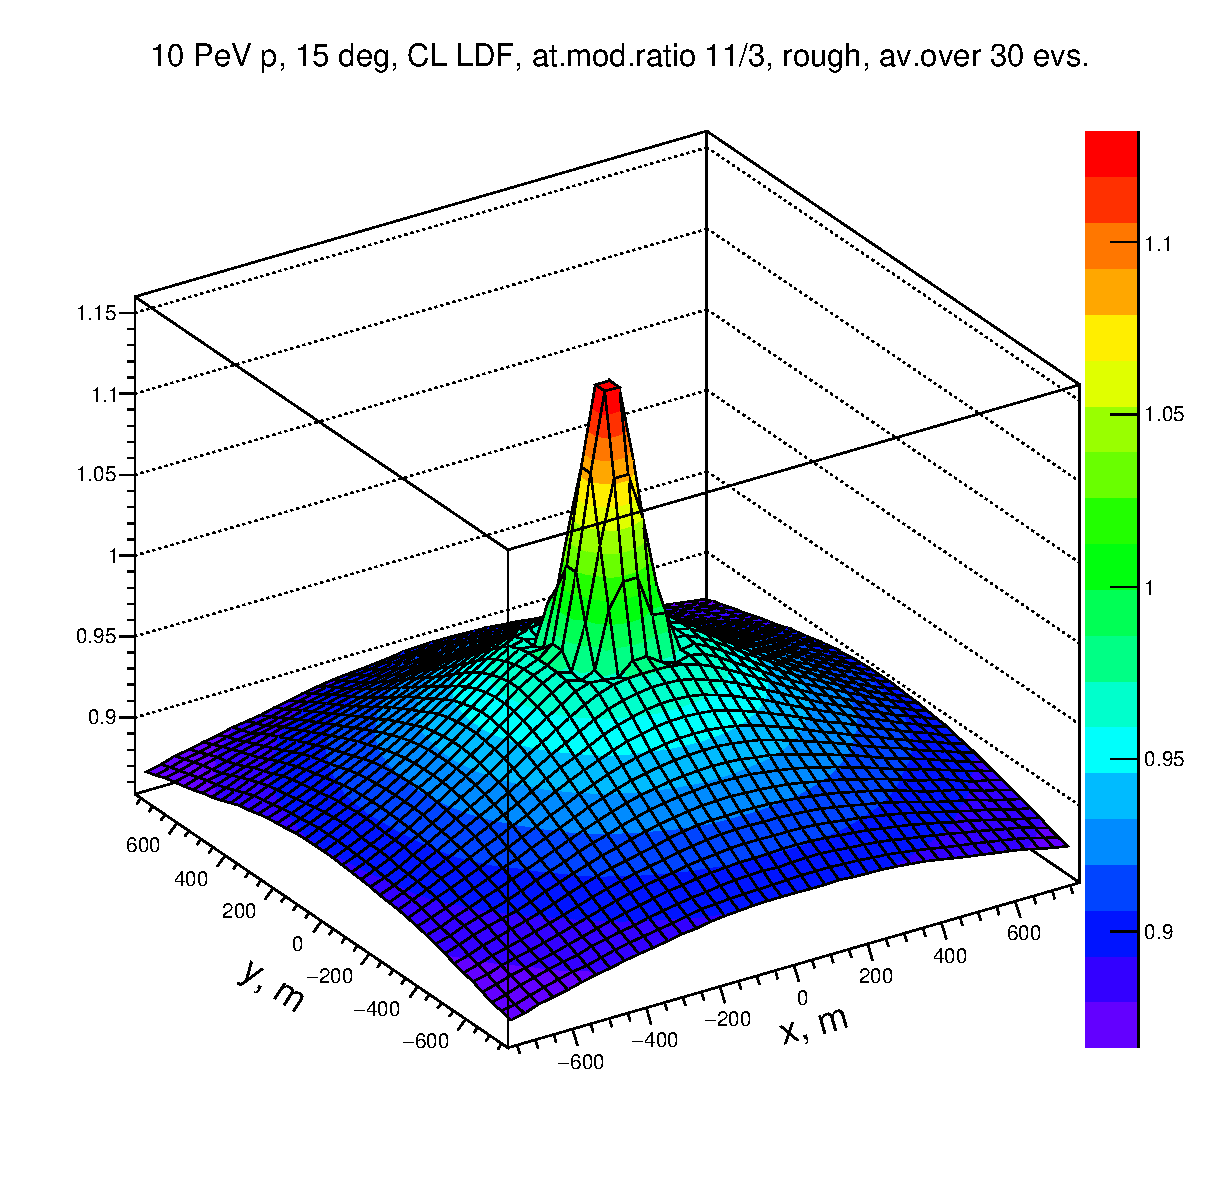
\includegraphics[width=19pc]{figs/11d3.eps}%
    \vspace{-1.0pc}
    \caption{Sample mean Cherenkov light lateral distribution ratio for CORSIKA atmosphere model
    pair 11/3. Bin size 50~m $\times$ 50~m. 10~PeV primary protons. Zenith angle 15~$\deg$. Sample volume 30~events.}
\label{fig:3d11}
\end{minipage}
\hfill
\begin{minipage}[t]{0.48\textwidth}
    \centering
    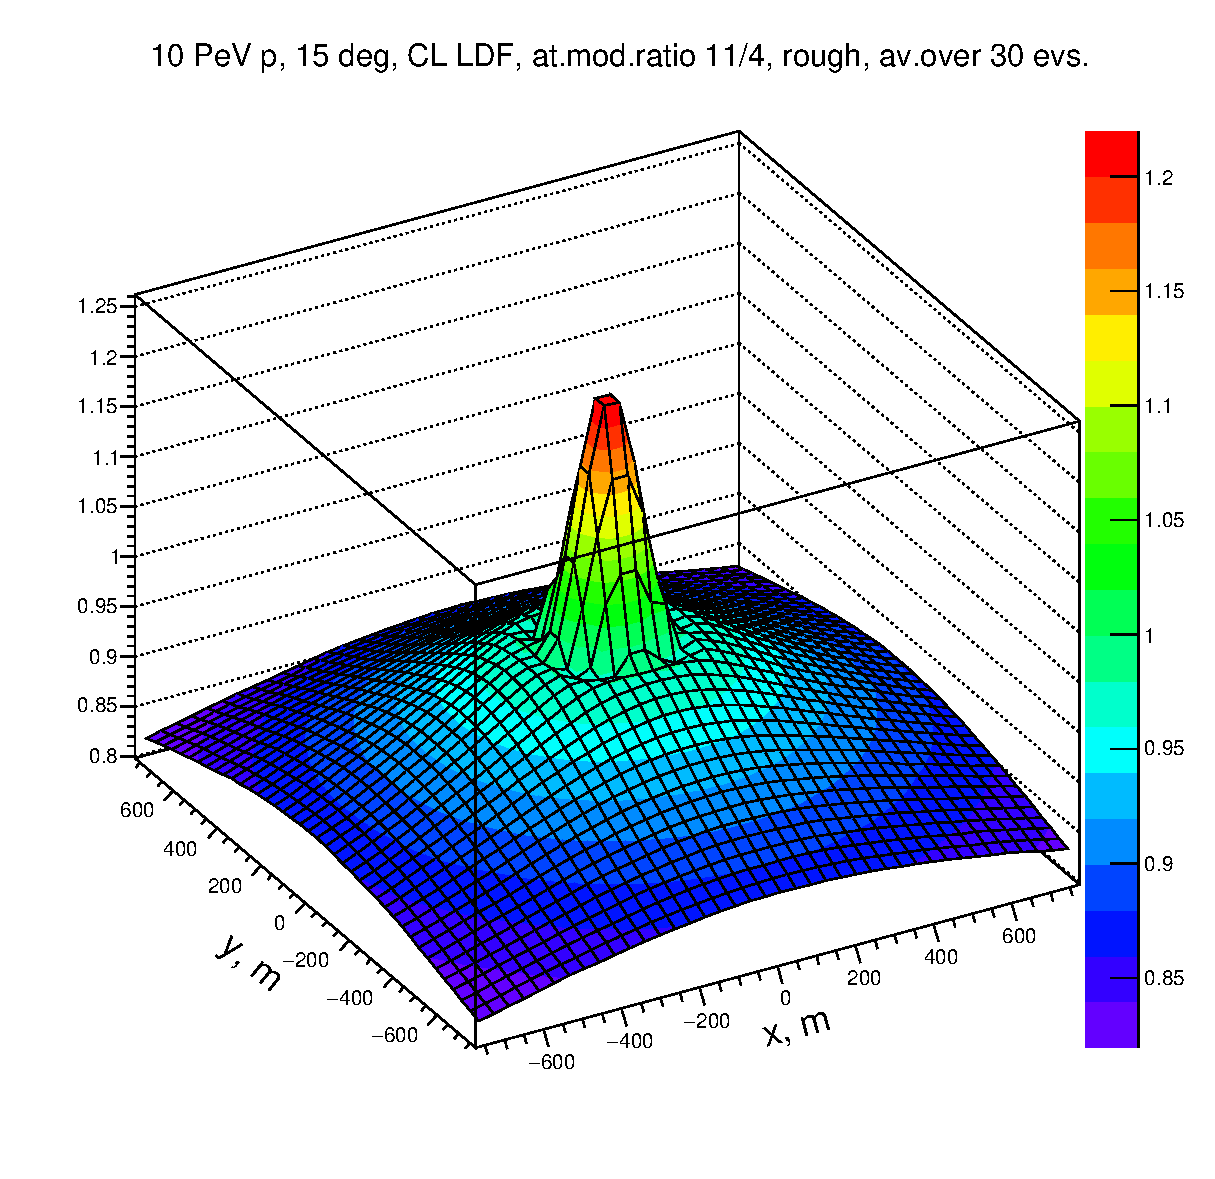
\includegraphics[width=19pc]{figs/11d4.eps}%
    \vspace{-1.0pc}
    \caption{Sample mean Cherenkov light lateral distribution ratio for CORSIKA atmosphere model
    pair 11/4. Bin size 50~m $\times$ 50~m. 10~PeV primary protons. Zenith angle 15~$\deg$. Sample volume 30~events.}
\label{fig:4d11}
\end{minipage}
\end{figure*}


CORSIKA atmosphere model 11 was used all through the modeling runs. Modeling lasted for about 2 years and at that time it was not possible to choose an atmospheric model close to reality. The use of the experimental points in $T$ or $\rho$ cannot provide a reasonable  choice of the model, it can only give us some clue as to what the model should be. Full-fledged choice must include data on vertical profile of atmosphere layer up to altitudes at least 20 km above the lake Baikal level because the Cherenkov light mostly comes from this layer. Still we can make some conclusions on the atmosphere model effect on primary energy and mass estimates by comparing the artificial showers simulated for different models.

We produced such artificial events initiated by 10~PeV protons for a number of models,  passing close to the experimental $T$ and $\rho$ trajectories, and CORSIKA model 11. The results are expressed as ratios of full numbers of Cherenkov photons and lateral distribution functions.
The lateral distributions were calculated within a vast (3.2km $\times$ 3.2km) carpet tyled with 2.5~m $\times$ 2.5~m squares but for the purpose of the comparison were smoothed by integrating over 50m $\times$ 50~m squares approximately imitating the sensitivity spots of telescope pixels.
Sample volume for each model was 30 showers. Table~\ref{tab:atmmod} shows mean values and variations of Cherenkov photon number ratios for three pairs of CORSIKA atmosphere models (3/4, 3/11 and 4/11). The ratios of sample mean lateral distributions for 3/11 and 4/11 pairs are shown in Fig.~\ref{fig:3d11} and Fig.~\ref{fig:4d11}, respectively. Pair 3/4 reflects maximum effect of atmosphere model choice from the viewpoint of experimental $T$ and $\rho$ measurements. Pairs 3/11 and 4/11 compare the model 11 used in simulations to the models approximating the experimental data.
Table data clearly states that substantial changes of atmosphere model affect the total number of Cherenkov photons and thus the primary energy estimates not more than by 5\% on average. Conclusions on primary mass estimates are not so clear but the lateral distribution ratio plots indicate some changes in CL LDF of about 6 to 12\% (12 to 20\%) near the shower core, closer than 80 m, and about -2 to +6\% (0 to +12\%) in 80-150m circle for 3/11 (4/11) pair, which definitely might affect our mass-sensitive criterion. More accurate evaluation of the effect will be given elsewhere.


%%%% === mosaic picture ===
%\begin{figure}[tb]
%\centering
%    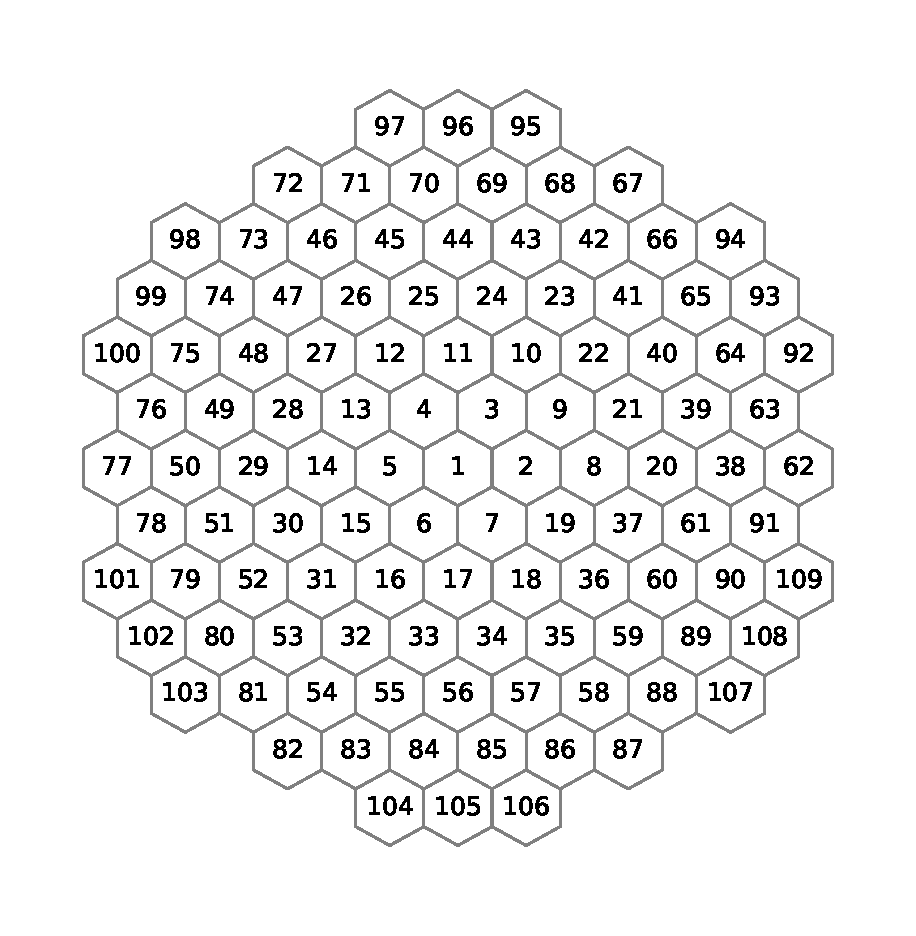
\includegraphics[width=19pc]{figs/mosaic.pdf}%
%    \vspace{-1.0pc}
%    \caption{The PMT mosaic of the SPHERE-2 detector with PMTs numbers indicated.\todoi{Грохнуть!}}
%\label{fig:mosaic}
%%\end{minipage}
%\end{figure}


%%% === PMT FOV picture %%%
\begin{figure*}[bth]
\centering
    %\includegraphics[width=0.44\textwidth, bb= 100 100 900 900,clip]{figs/fov.eps}\hspace{2pc}%
    \includegraphics[width=0.9\textwidth]{figs/fov.pdf}
    %\vspace{10pt}
    %\includegraphics[width=0.49\textwidth]{figs/fov_log.eps}%
    \caption{The PMTs' fields of view for detector at altitude $H=$ 1000~m. There are presented calculated FOV of PMTs 1, 5, 14, 29, 50 and 77 as indicated on the Fig.~\ref{fig:2012-3_shore_image} in assumption of vertical detector optical axis position. The inclinations of the PMTs axis from the SPHERE detector optical axis change from 0 to 26 degrees uniformly.}
\label{fig:pmt_fov}
\end{figure*}


\subsection{PMTs' field-of-views correction}

In flight during measurements whenever the detector become inclined, the configuration of it's field-of-view (FOV) changed. The FOV of some PMTs shrunk and got closer to the central PMT FOV, for others got larger and moved further from the central PMT FOV. This distorted the reconstructed Cherenkov LDF in spatial terms. Also, change in FOV orientation meant change in optical distance from which the PMT collects light (which affected time measurements). Another issue was the relevant change in average angle under which the snow surface was observed by PMT, which changed light scattering effectiveness (and this distorted the LDF in terms of signals values). In other words, the mosaic inclination if compared to the ground based experiments resulted in measuring stations repositioning with grid distortion and in gradual change in stations sensitivity.

In addition to the full Monte Carlo simulation of the SPHERE detector described in~\cite{Ant19} the calculations of detector's optics and PMTs' FOV was performed. The detectors optical scheme is presented on the Fig.~\ref{fig:optics}. % здесь надо другую схему, нежели ту, что была. 

\begin{figure}[bth]
\centering
    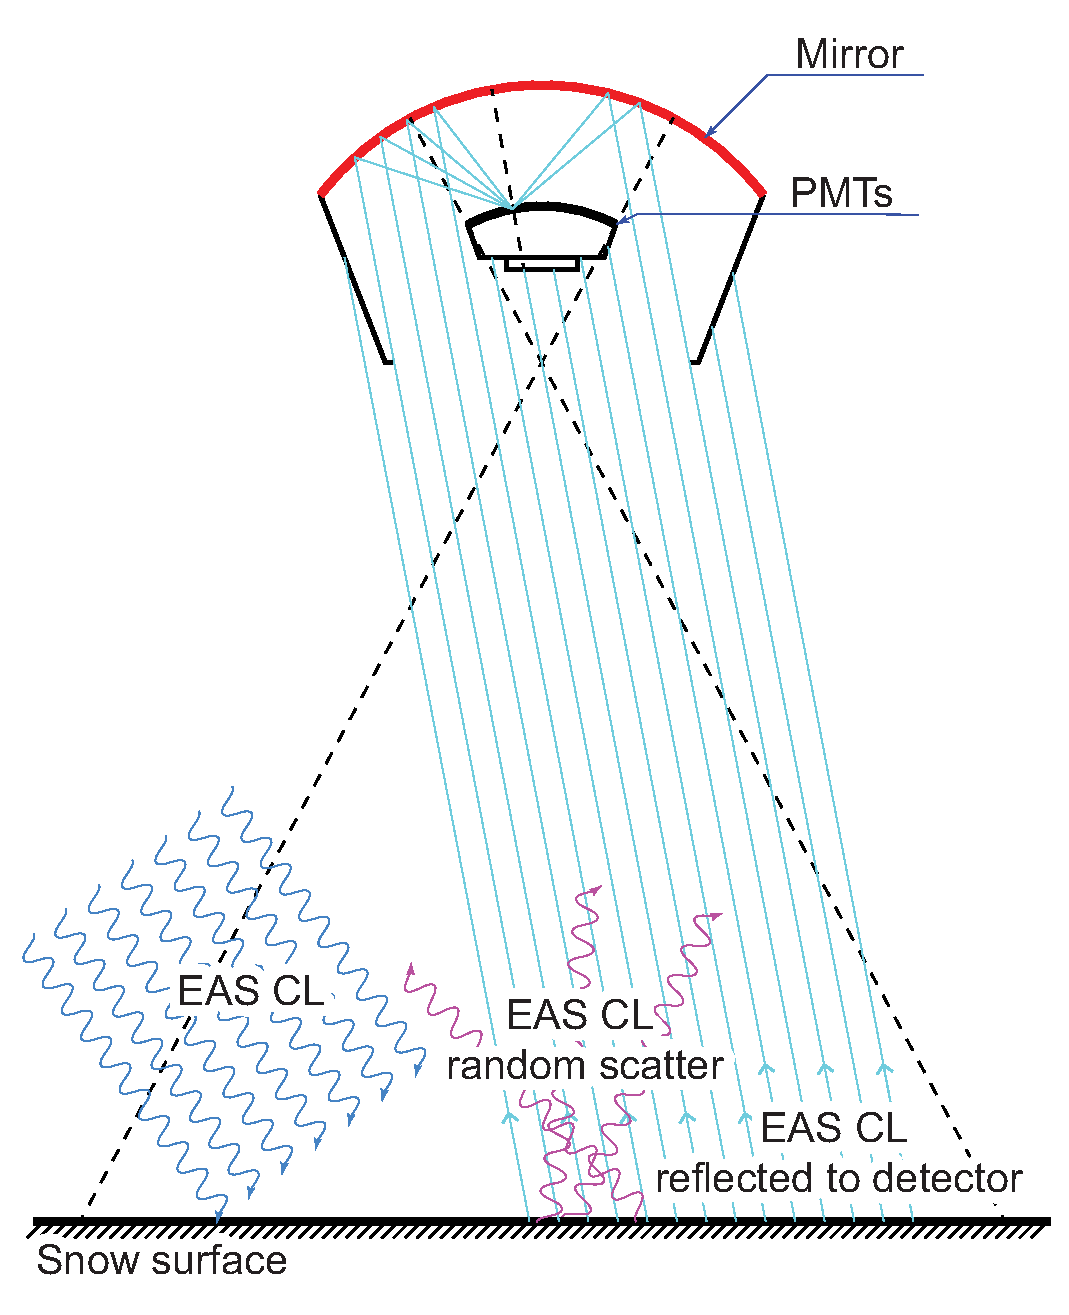
\includegraphics[width=0.45\textwidth]{figs/optics.eps}
    \caption{The detector optical scheme.}
\label{fig:optics}
\end{figure}

\todoi{Сократить}
The detector was set at 1000~m altitude with zero inclination above flat horizontal observation level. The ground level was divided by the square mesh $[X;Y]$ with 1~m step. From each ground square the weighted photons were emitted towards the detectors diaphragm. The diaphragm was divided into $[x;y]$ mesh with 5~mm step. From each ground square a total of 25600 photons were emitted towards the detector. Each photon weighted by the snow reflection coefficient $k_{snow}$ (taken as 0.95~\cite{war82}), by the $\cos^2(\theta)/2$ to account for Lambert scattering (the $\theta$ is the angle between the direction to the detector and Z-axis), by the distance factor $2\pi{}S/(H^2+(X-x)^2+(Y-y)^2)$ and additional $\cos\theta$ to account the non-normal ray incidence on the diaphragm {\color{red}plus} the normalization coefficient of 2.

At the detector diaphragm level the photons were checked whether they passed the the diaphragm successfully or not and were traced further. At the mosaic level (the mosaic geometrically is a domed {\color{red}tflightcated} cone) the photons were checked that they missed back side of the mosaic and were traced further to the mirror. At the mirror the photons were reflected and additionally weighted by the mirror reflection coefficient $k_{mirr}$. During different seasons of observations this coefficient changed as the mirror degraded, so for data analysis the coefficients were selected accordingly to {\color{red} measured ones}, $k_{mirr}$ was about 0.75--0.80 during 2011--2012 seasons and $k_{mirr}$=0.95 for the new mirrors in 2013. After the photons were reflected by the mirror, they were traced back to the mosaic level and check for successfully hitting it. At this step the photons were checked whether they hit any PMT or mosaics blind material. The \mbox{FEU-84-3} PMT's photocathode has 26~mm diameter sensitive area. The spacing between photocathode centers in out mosaic was 44.5~mm, so only 30\% of the mosaic was sensitive to the light. For each photon at the PMT glass surface the glass mirroring coefficient $k_{PMT}$ was calculated, the photon's polarization was selected randomly.

Tracing photons from the full ground grid allowed to find each PMT's FOV and to determine the light collection efficiency for each point on the ground (e.g. how many of the photons that reach the snow surface will be collected by the detector).
Fig.~\ref{fig:pmt_fov} shows the field of view of PMTs with different deviation angles  from the detector optical axis in an assumption of vertical detector optical axis position. There are presented calculated FOV for PMTs with numbers 1, 5, 14, 29, 50, 77 as they are indicated on the Fig.~\ref{fig:2012-3_shore_image}. The declination angles of presented PMTs change from 0 to 26 degrees in dependence of the PMT's distance from PMT mosaic center on Fig.~\ref{fig:2012-3_shore_image}. The PMT1 is the Hamamatsu R3886 PMT that has the larger photocathode sensitive area than others FEU-84-3 PMTs, it is seen clearly on the Fig.~\ref{fig:pmt_fov}. 

The same calculations was made for the detector position with different detector axis inclination angles. From the known PMT FOV the coordinates for FOV center were obtained and later used in shower arrival direction reconstruction and shower axis location.


\section{Conclusions \label{sect:conclusions}}

%{
%\Russian

%В статье мы описали как в эксперименте мы измеряем параметры установки  СФЕРА-2, важные для восстановления черенковских событий.  В частности, высота установки над уровнем земли измеряется двумя способами, что позволяет определить истинное значение высоты. Мы видим, что установка стабильна в воздушном потоке.
%} 
In the paper we demonstrated how the monitoring of the SPHERE-2 parameters works. 

%{
%\Russian
%Зарегистрированный установкой сигнал очищается от аппаратных эффектов. Мы выявили и учли импульсный шум аппаратуры каналов, влияние звездного фона. 

%Зарегистрированные события подверглись классификации. Из них выделены события от черенковского света ШАЛ. 
%}
The EAS event selection procedure is described.

%{
%\Russian
%Процедура восстановления параметров ШАЛ будет описана в последующих публикациях.
%}

\section{Acknowledgments}
We are grateful to the Lebedev Physical Institute of Russian Academy of Sciences group (leader S.B.~Shaulov) for assistance in assembling and testing the electronic equipment and in preparation of expeditions. We also thank the Baikal-GVD collaboration and G.V.~Domogatsky (Institute for Nuclear Research, Russian Academy of Sciences) for the support of the SPHERE experiment at the Baikal Lake scientific station.

%%%%%%%%%%%%%%%%%%%%%%%%%%%%%%%%%%%%%%%%%%%%%%%%%%%%%%%%%%%%%%%%%%%%%%%%
\section{References}
\bibliography{Sphere-Data.bib}

\end{document}